\chapter{User Interface Design}

DREAM is a web-based application. It could be utilized on a variety of devices, independent of form factor. The application, however, is expected to be largely utilized on desktop computers. As a result, the given mockups depict representations of the application's desktop version.

This chapter provides pictures of all the  mockups, that will be later used for the requirements traceability (see chapter \ref{ch:requirements_traceability}).

\subsubsection{Unregistered user}

User's registration screen, allowing user to provide all data necessary for account creation. The user can navigate to this screen via \textit{Create account} option, available in the horizontal navigation bar on the top of the page. After correctly filling the form, the user is redirected back to the home page and receives a notification informing him about the success of the account creation process.
\begin{figure}[H]
\centering
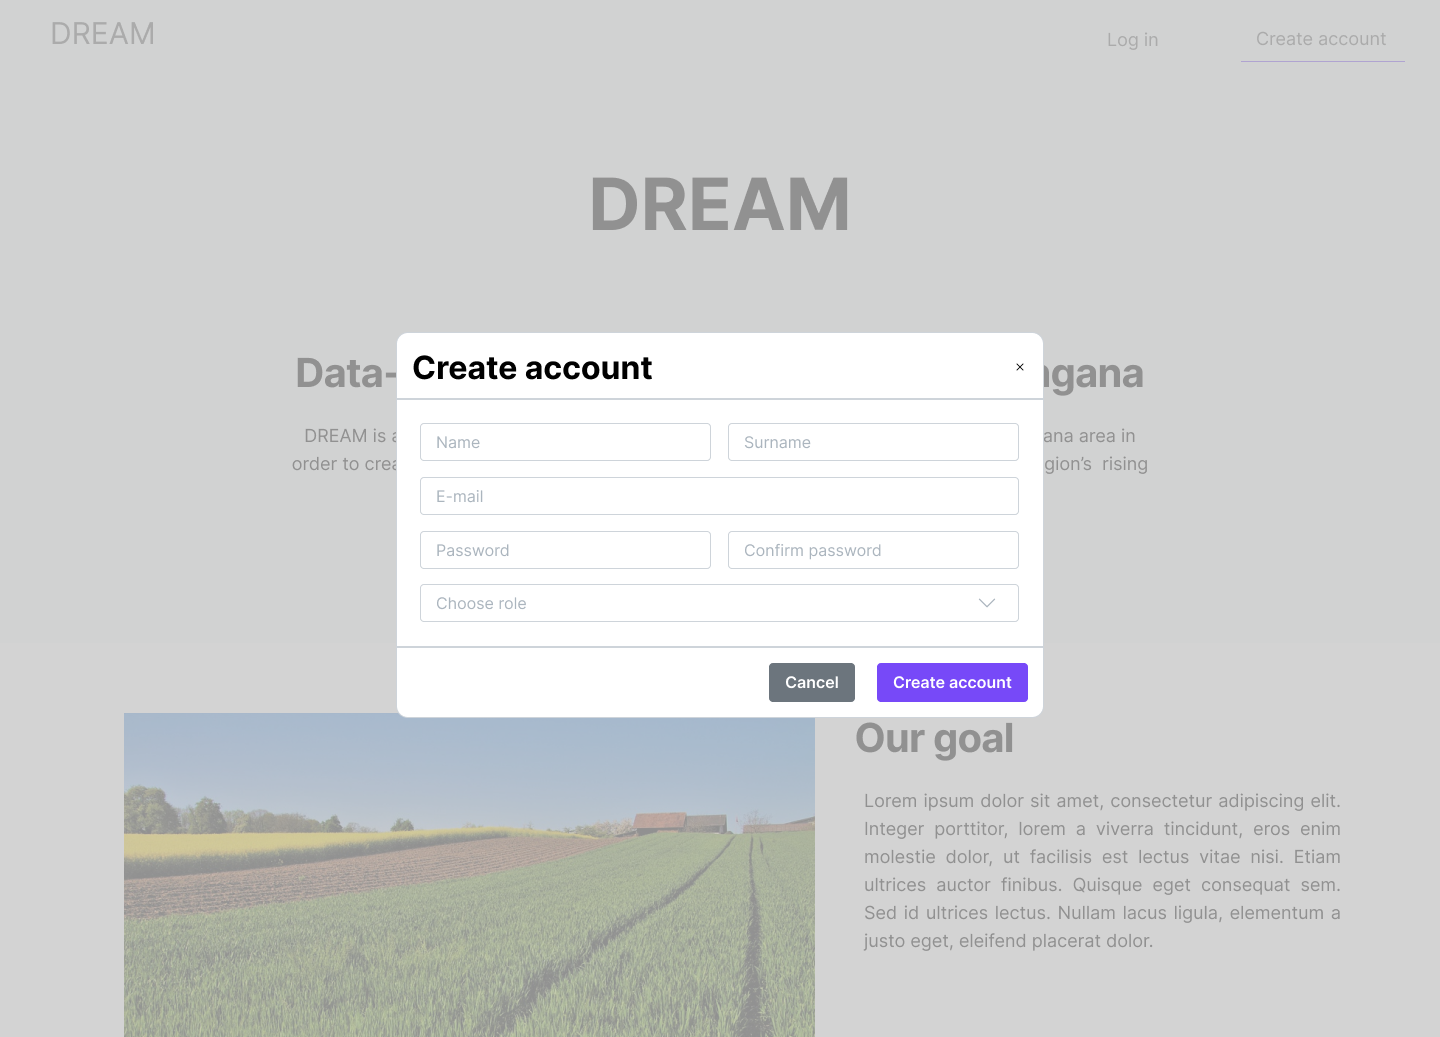
\includegraphics[width=0.75\textwidth]{mockups/Unreg. user_Create account.png}
\caption{\textbf{M1.} User registration.}
\end{figure}

User's registration screen, after choosing \textit{Famer} role. Additional fields appear, specific to the Farmer role, namely Sensor system's ID, Water irrigation system's ID, Address line 1, Address line 2, Postal code, City, and Mandal.
\begin{figure}[H]
    \centering
    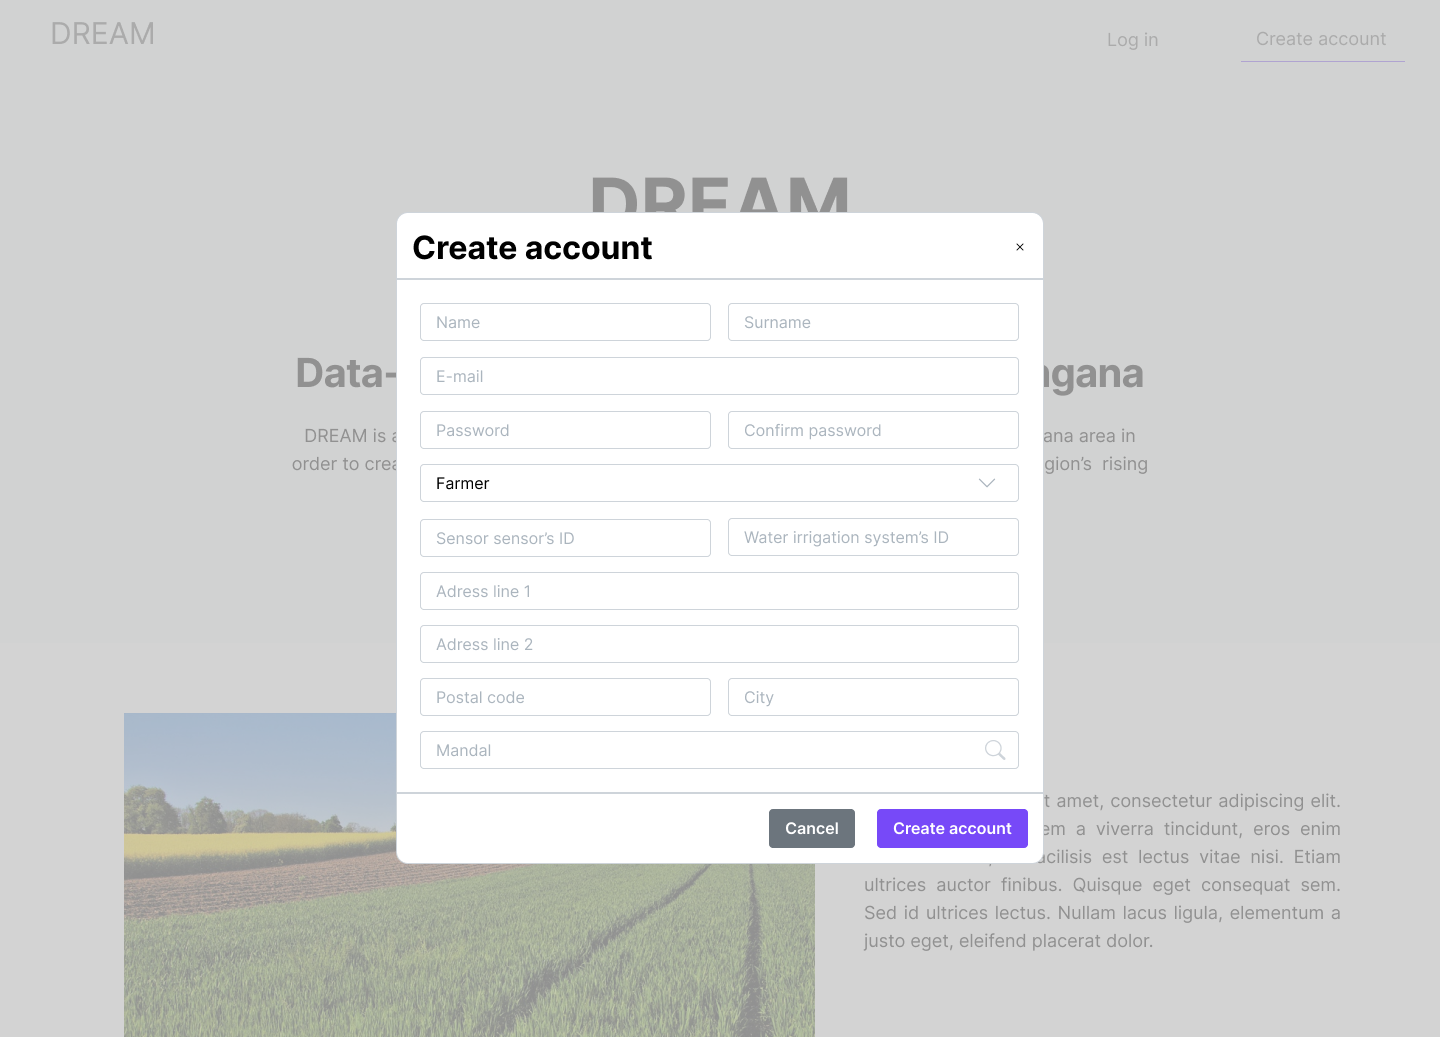
\includegraphics[width=0.75\textwidth]{mockups/Unreg. user_Create account_Farmer.png}
    \caption{\textbf{M2.} Farmer registration.}
\end{figure}

User's registration screen, after choosing \textit{Agronomist} role. Additional fields appear, allowing to choose the area of responsibility.
\begin{figure}[H]
    \centering
    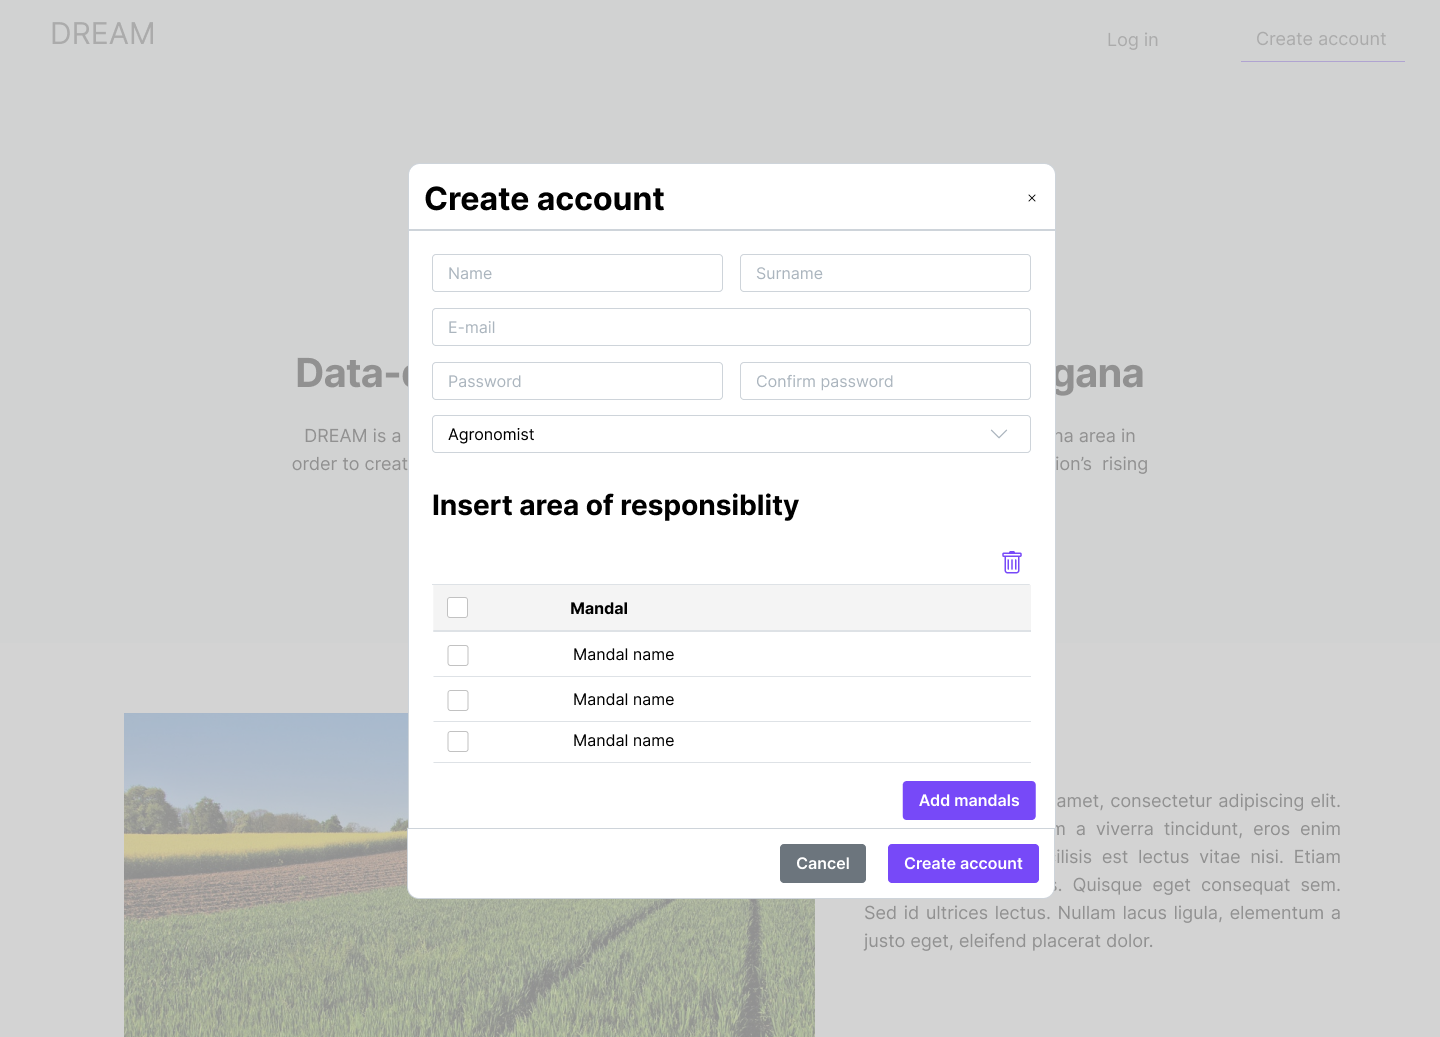
\includegraphics[width=0.75\textwidth]{mockups/Unreg. user_Create account_Agronomist.png}
    \caption{\textbf{M3.} Agronomist registration.}
\end{figure}

User's log in screen, allowing user to provide all data necessary for logging into the application, namely e-mail and password. The user can navigate to this screen via \textit{Log in} option, available in the horizontal navigation bar on the top of the page. User can also choose an option to remind a password, via a button in the lower part of the modal dialog.
\begin{figure}[H]
    \centering
    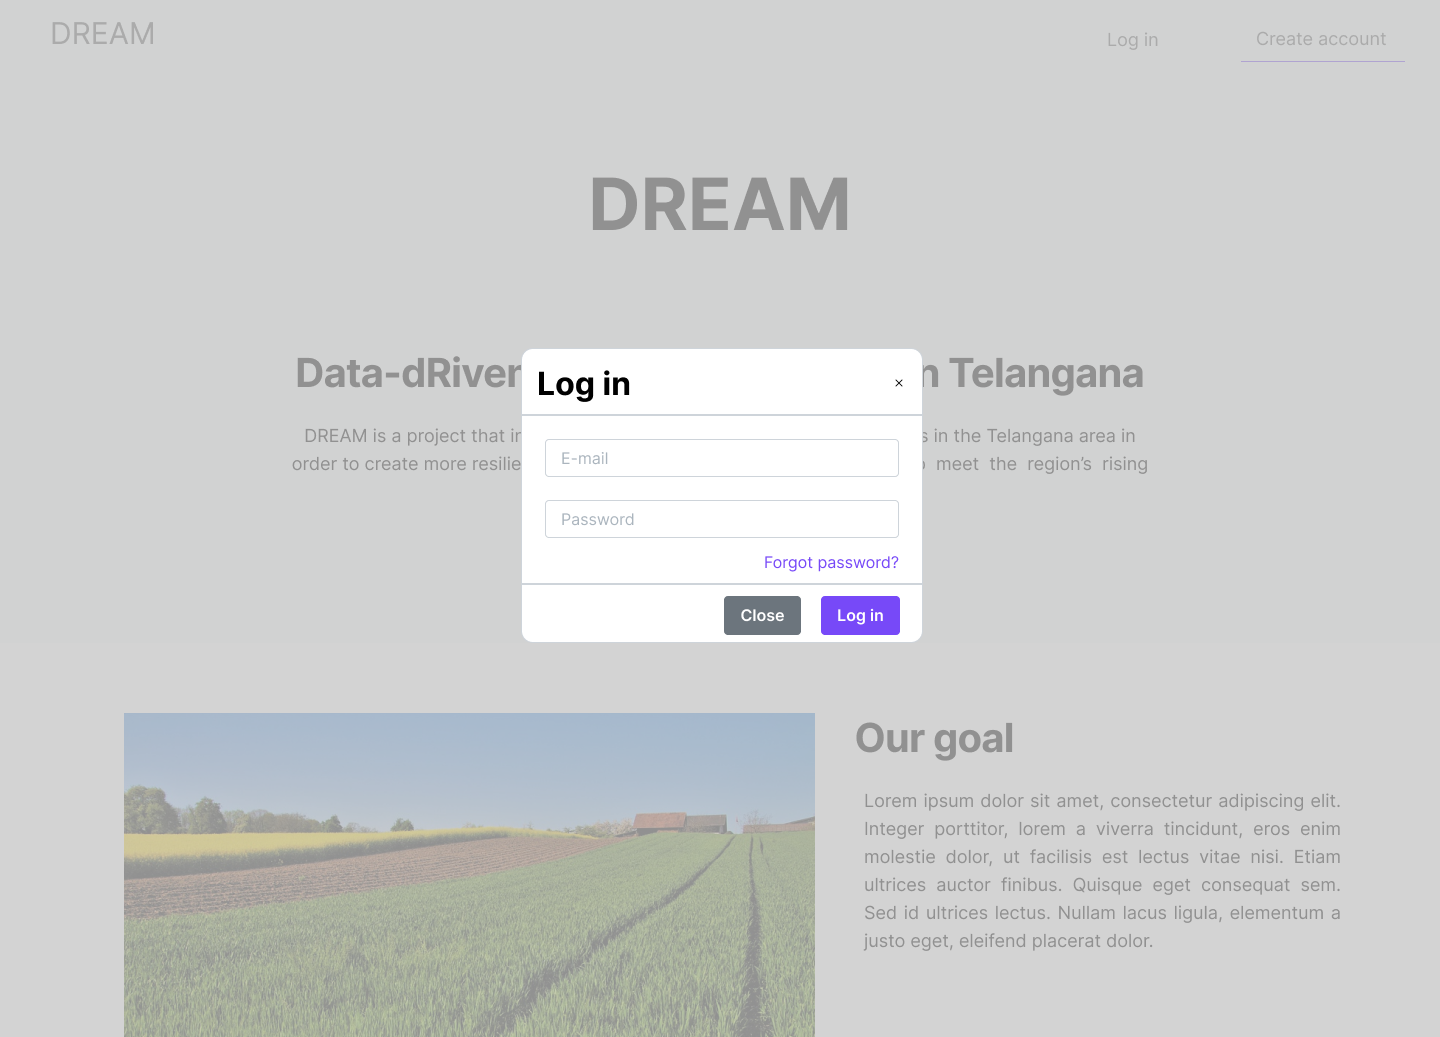
\includegraphics[width=0.75\textwidth]{mockups/Unreg. user_Log in.png}
    \caption{\textbf{M4.} Log in view.}
\end{figure}

User's remind password screen. The user can provide his e-mail address and click \textit{Remind} button, which sends a message to the provided address, containing a link, which allows resetting the password. If the user provides an e-mail address, that isn't in the database, the e-mail won't be sent. \todo{To powinno być w requirements :/}
\begin{figure}[H]
    \centering
    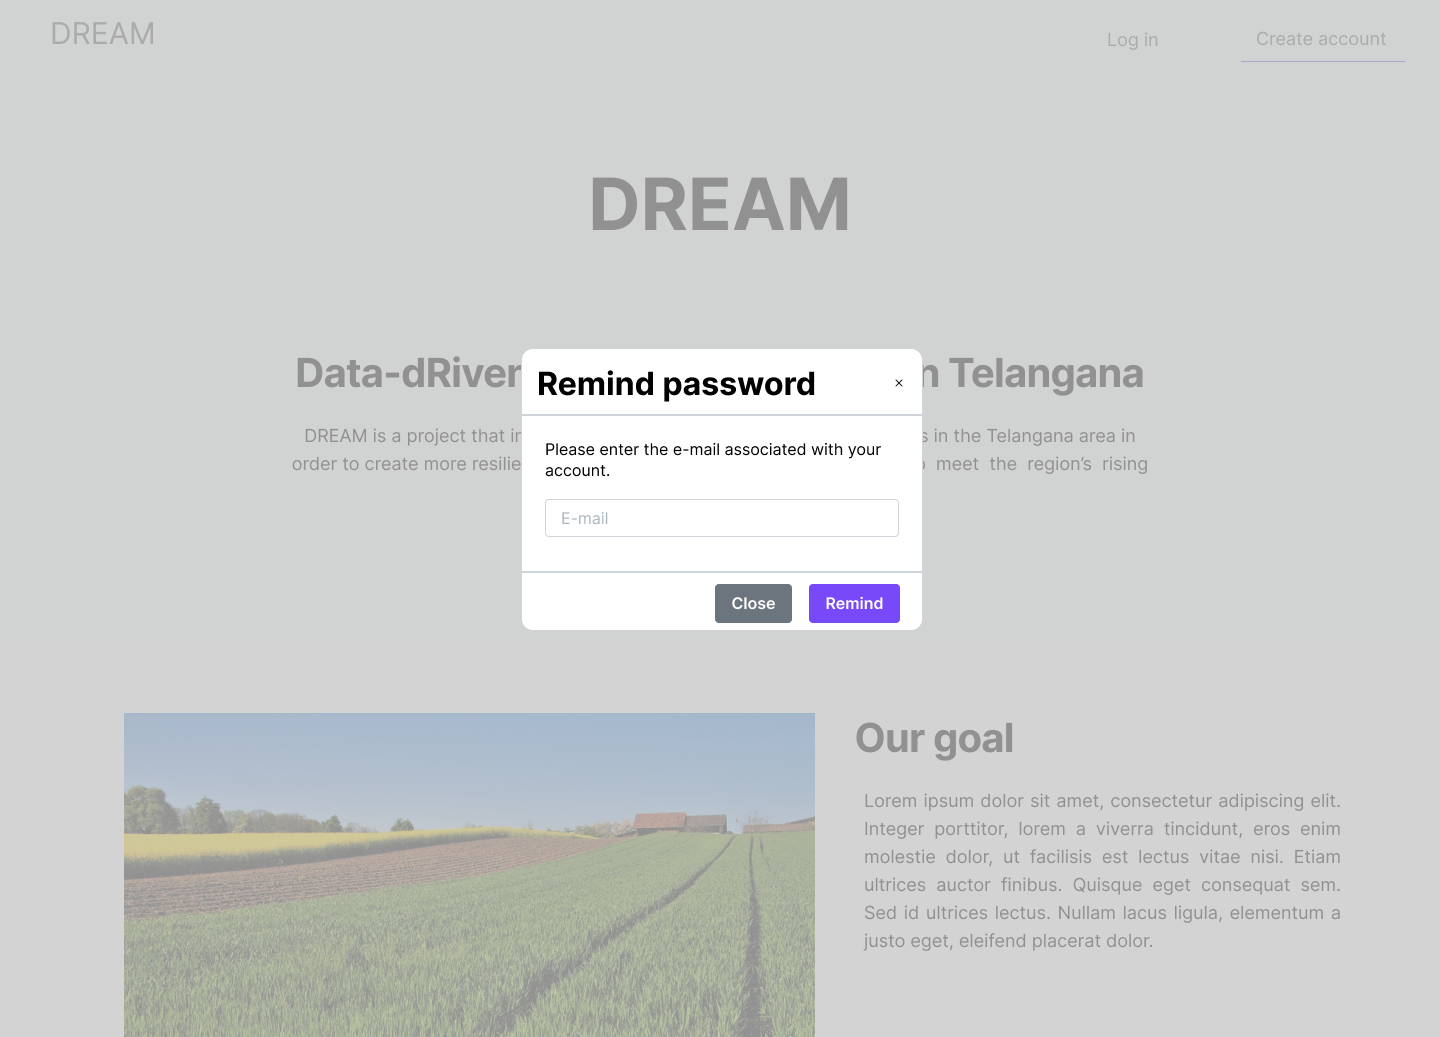
\includegraphics[width=0.75\textwidth]{mockups/Unreg. user_Remind password.png}
    \caption{\textbf{M5.} Remind password.}
\end{figure}


\subsubsection{Farmer}

Regardless of current view, a farmer can navigate to his summary, by clicking on the button containing his name and surname in the top navigation bar. The summary contains all the information about his account, and farm. Following information are provided: account data, note history, production data, farm visits, weather, soil humidity, water usage, and help requests. User can see detailed view about farm visits and help requests, by clicking on the eye button in  a given table row. Farmer can also delete his account, using the \textit{Delete account} button in the bottom of the page and after confirming his choice in a modal pop-up. 
\begin{figure}[H]
    \centering
    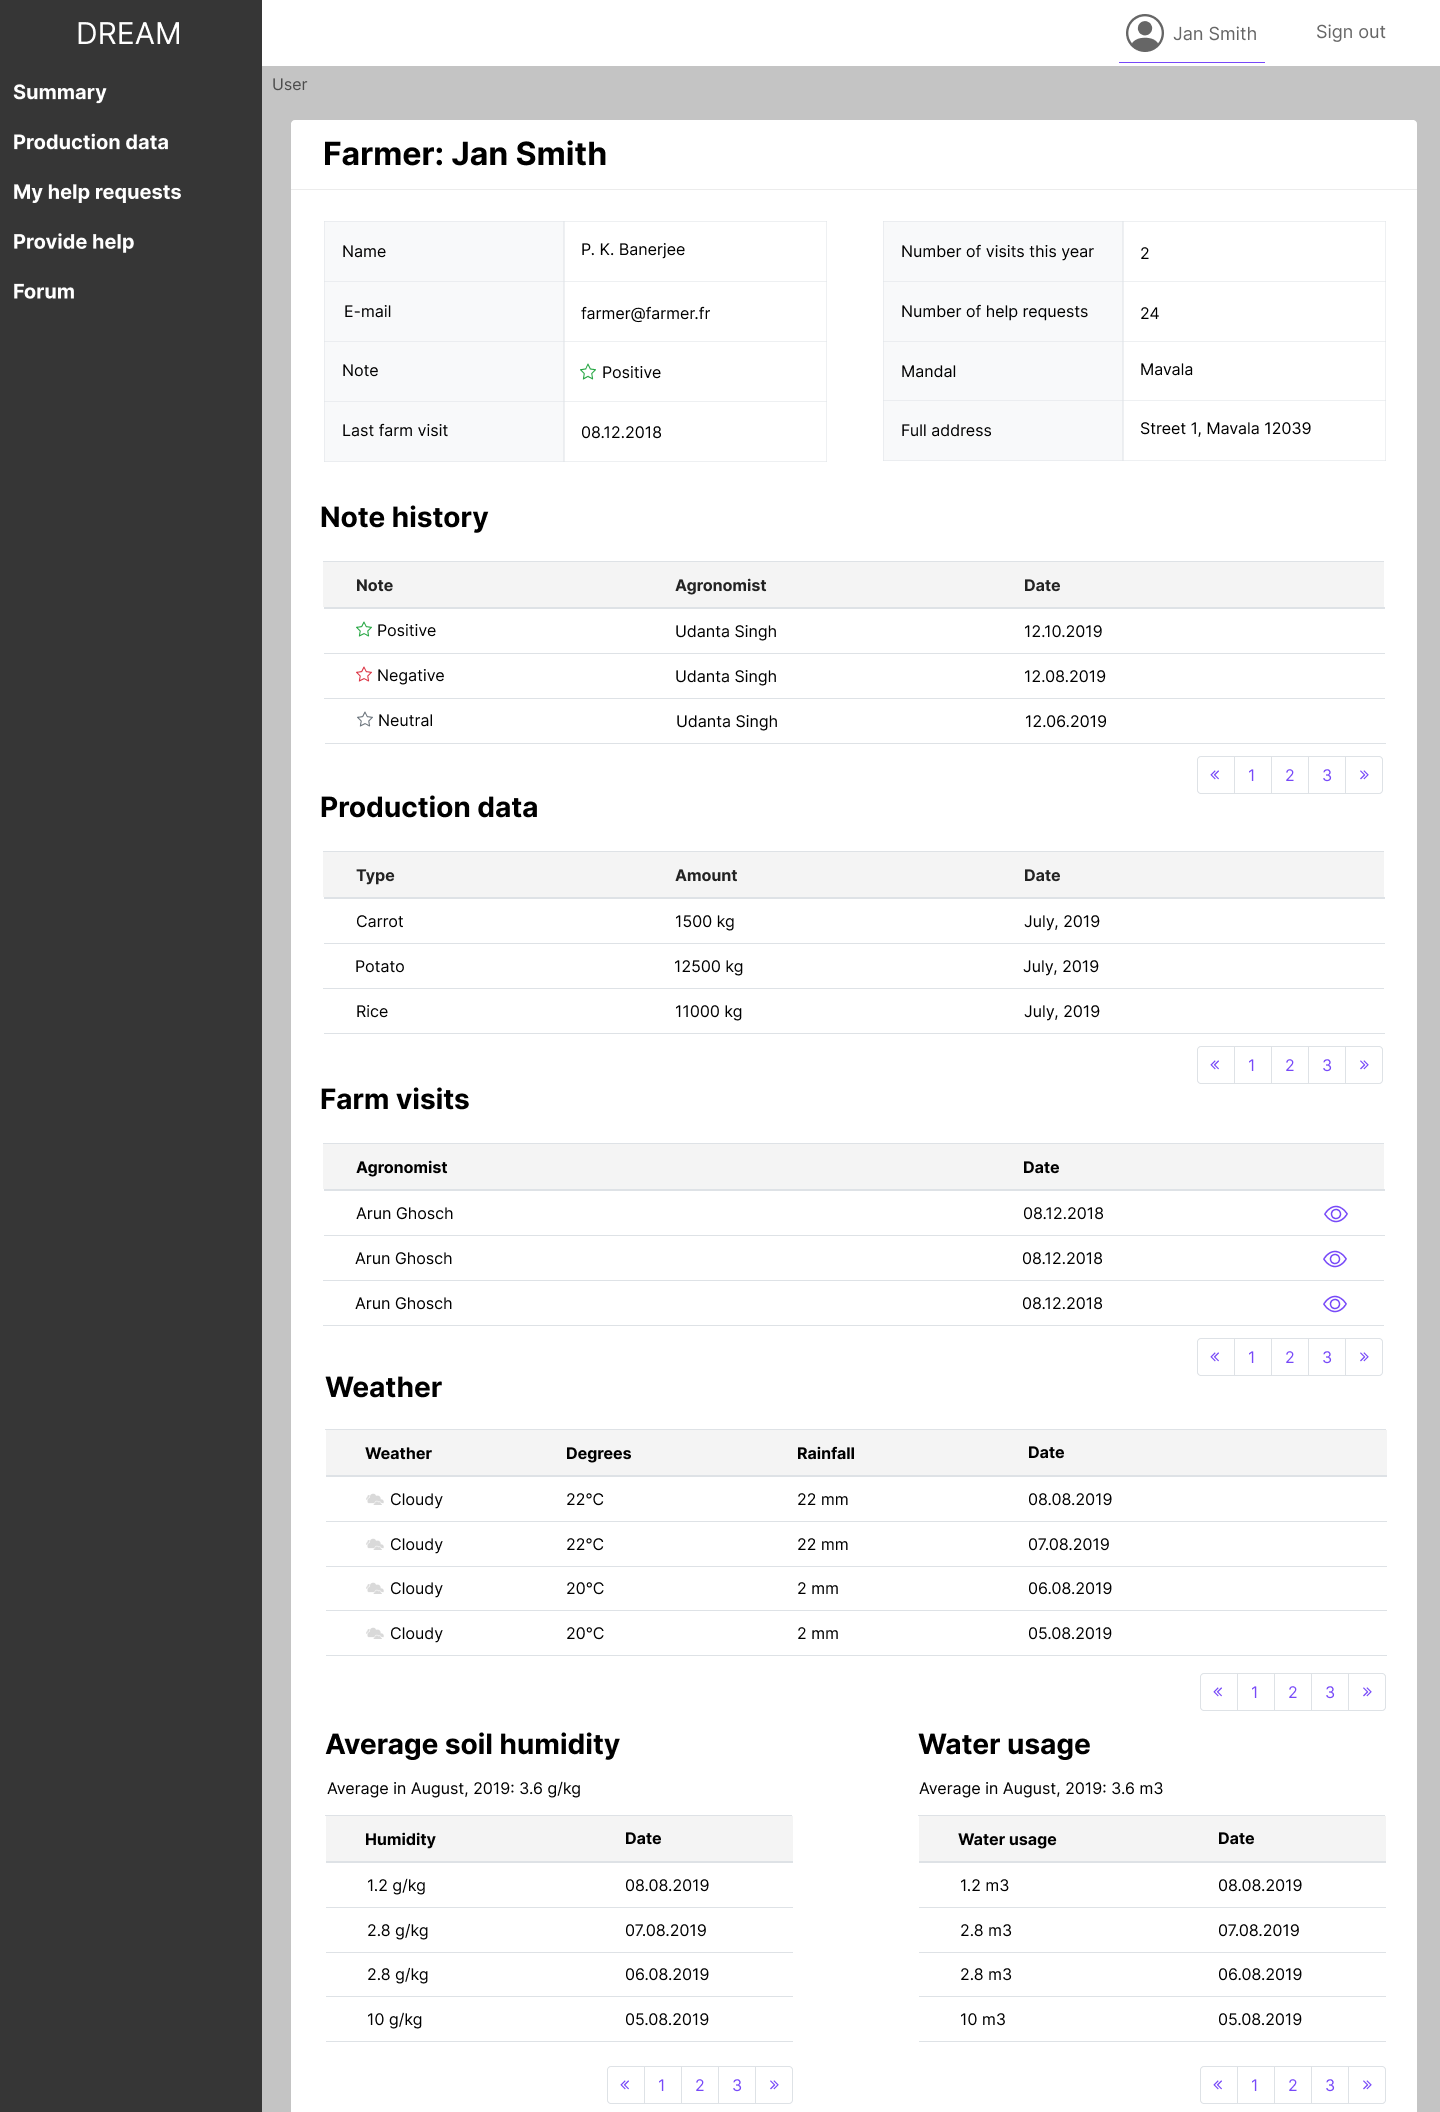
\includegraphics[width=0.75\textwidth]{mockups/Farmer_User_part1.png}
    \caption{\textbf{M6.1.} Farmer's user view - part 1.}
\end{figure}
\begin{figure}[H]
    \centering
    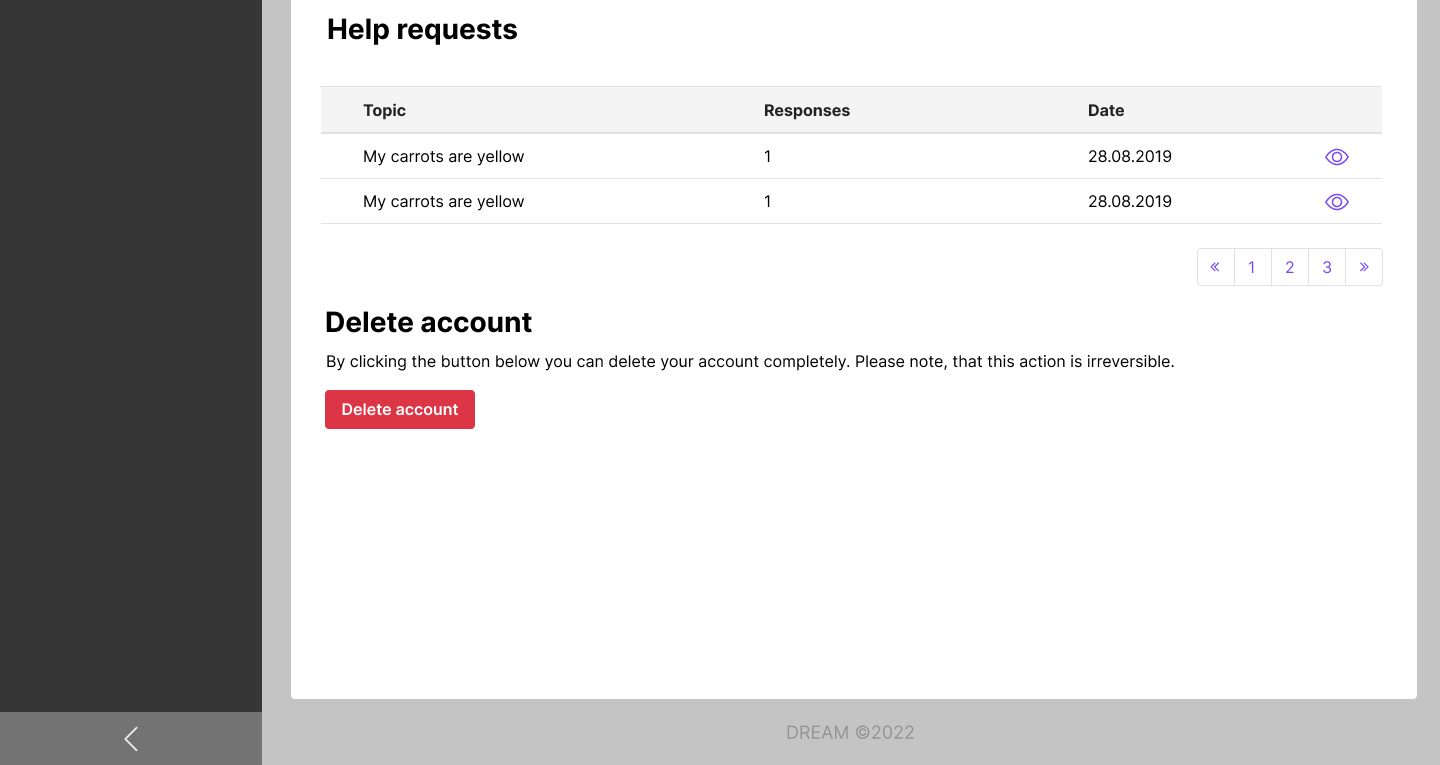
\includegraphics[width=0.75\textwidth]{mockups/Farmer_User_part2.png}
    \caption{\textbf{M6.2.} Farmer's user view - part 2.}
\end{figure}

Directly after logging in, farmer is forwarded to the dashboard page, containing a summary of the most important information. From there he can navigate to other views by the navigation bar in the left part of the page, the navigation bar in the upper part of the page or by clicking on the button in the lower part of some summary cards.  
\begin{figure}[H]
    \centering
    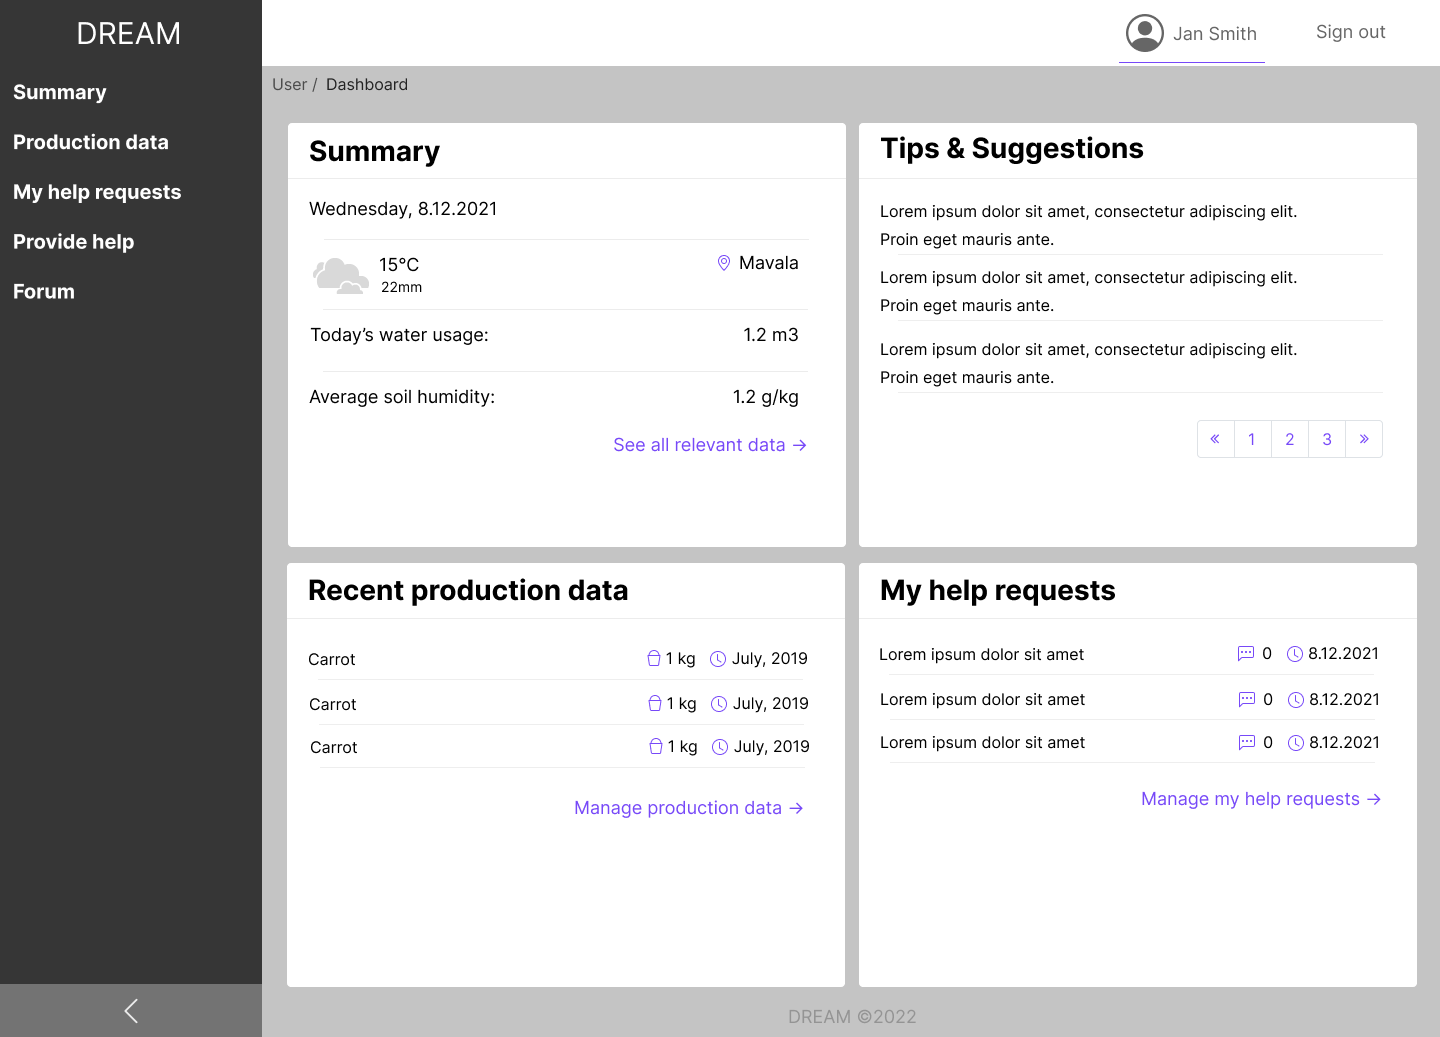
\includegraphics[width=0.75\textwidth]{mockups/Farmer_Dashboard.png}
    \caption{\textbf{M7.} Farmer's dashboard.}
\end{figure}

The farmer can manage his production data, by choosing the option \textit{Production data} in the left navigation bar. The production data view consists of a table with the latest data, an \textit{Add new} button and an option to delete previously provided information. After clicking on the \textit{Add new} button, a modal dialog appears, allowing the farmer to create a new entry.
\begin{figure}[H]
    \centering
    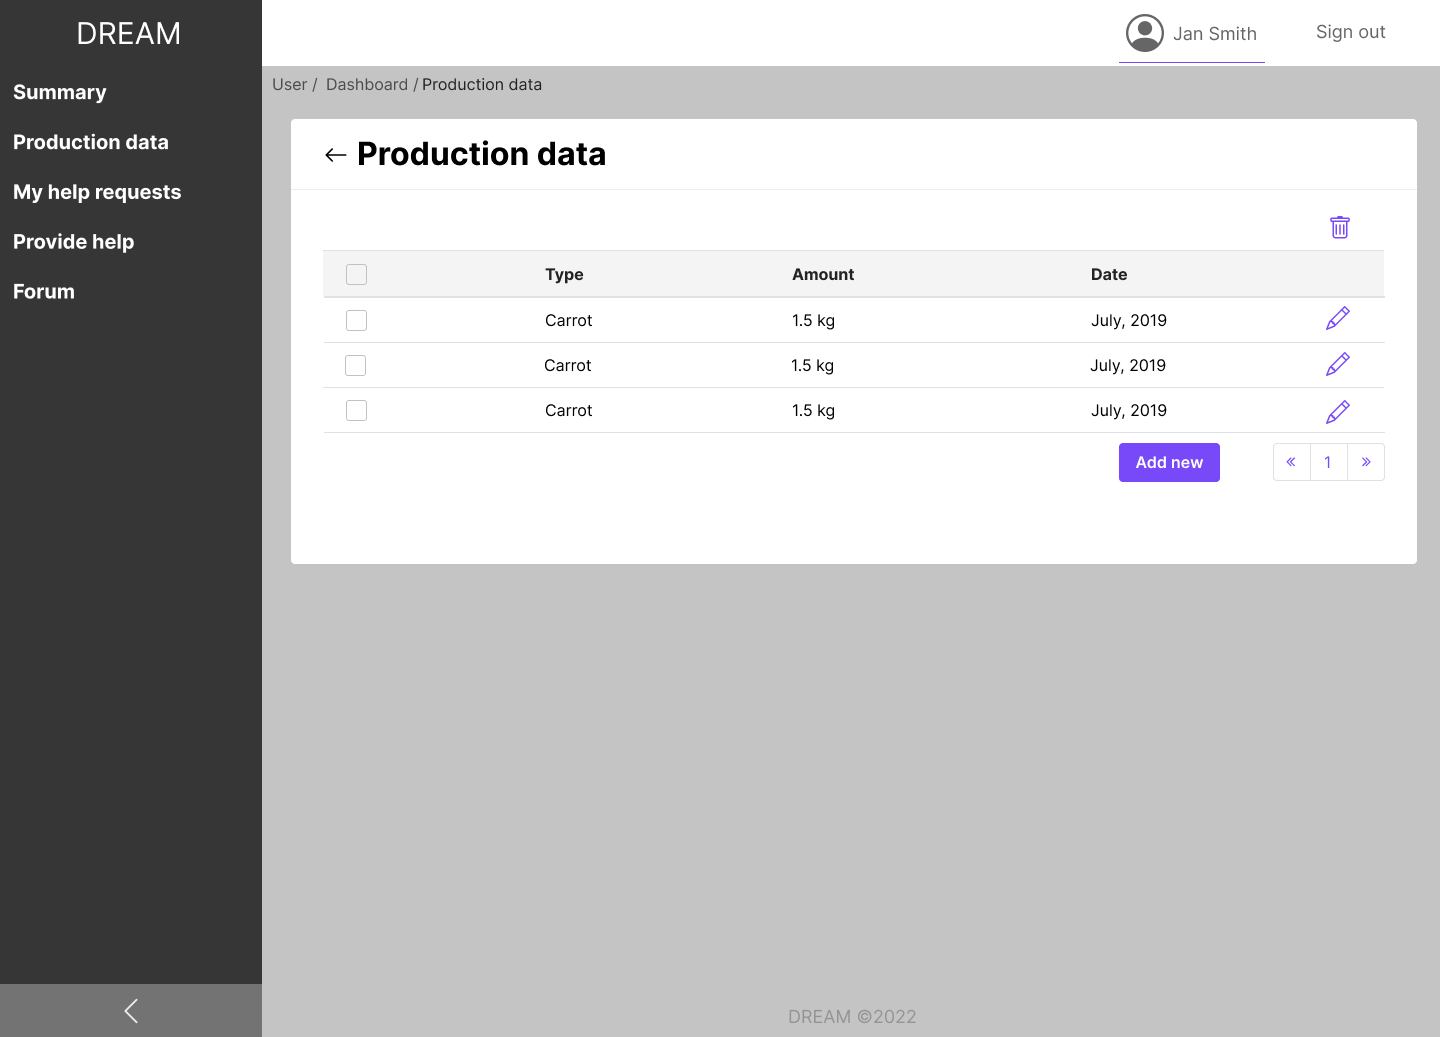
\includegraphics[width=0.75\textwidth]{mockups/Farmer_Dashboard_Production data.png}
    \caption{\textbf{M8.} Farmer's production data.}
\end{figure}

\begin{figure}[H]
    \centering
    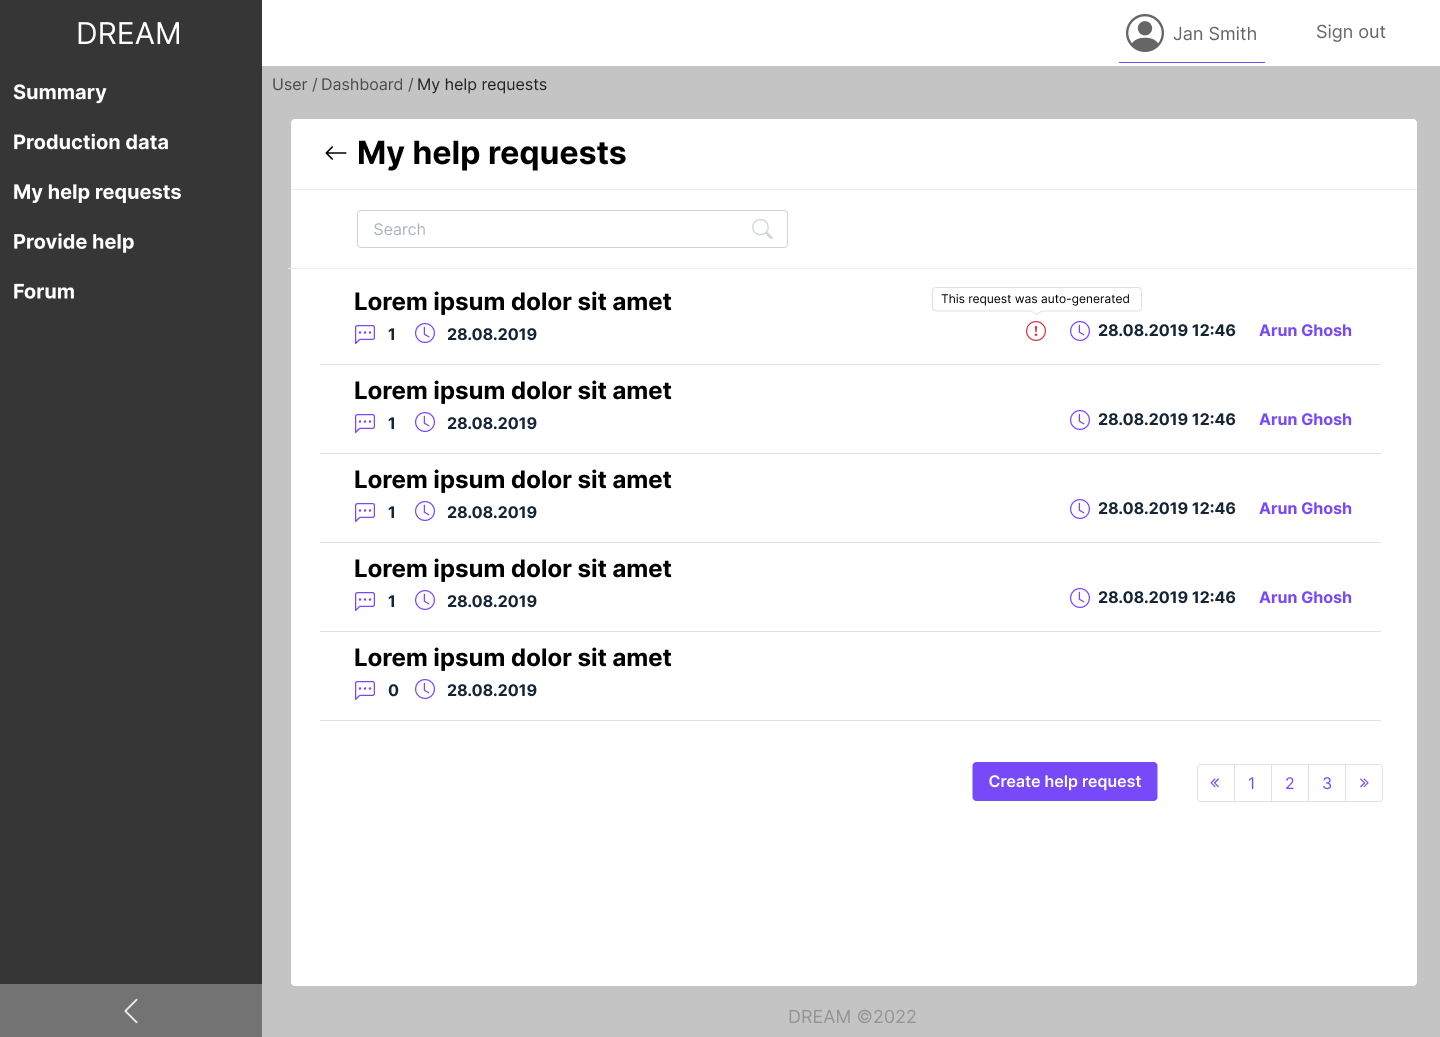
\includegraphics[width=0.75\textwidth]{mockups/Farmer_Dashboard_My help requests.png}
    \caption{\textbf{M9.} Help requests created by farmer.}
\end{figure}

\begin{figure}[H]
    \centering
    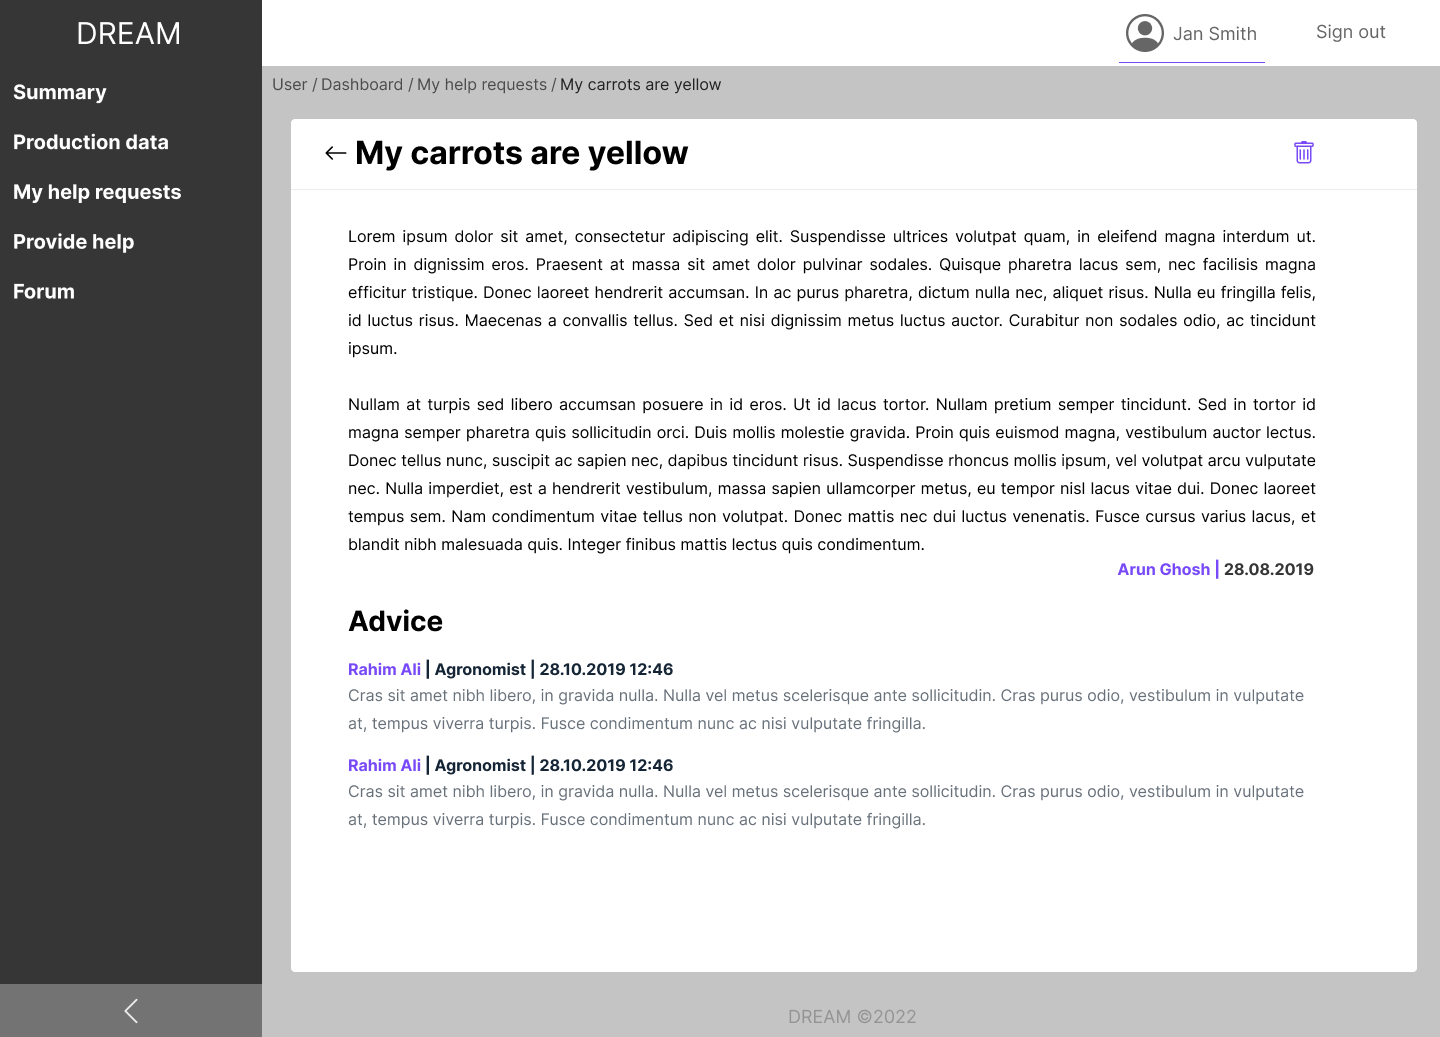
\includegraphics[width=0.75\textwidth]{mockups/Farmer_Dashboard_My help requests_VIew request.png}
    \caption{\textbf{M10.} Specific help request created by farmer.}
\end{figure}

\begin{figure}[H]
    \centering
    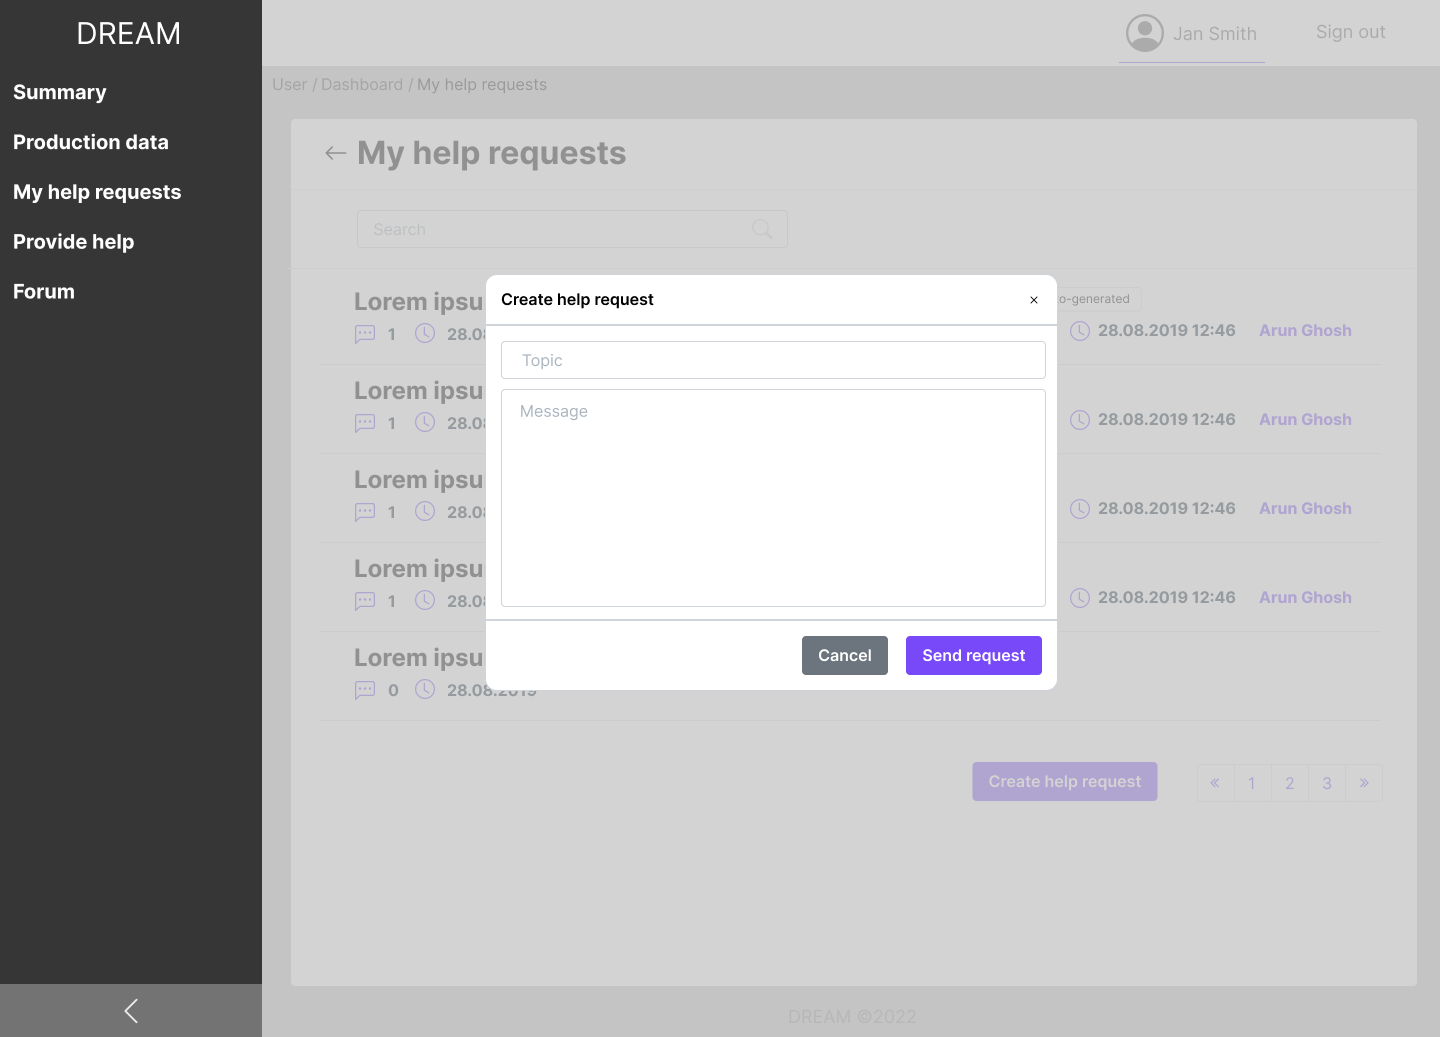
\includegraphics[width=0.75\textwidth]{mockups/Farmer_Dashboard_My help requests_Create help request.png}
    \caption{\textbf{M11.} Creating help request.}
\end{figure}

\begin{figure}[H]
    \centering
    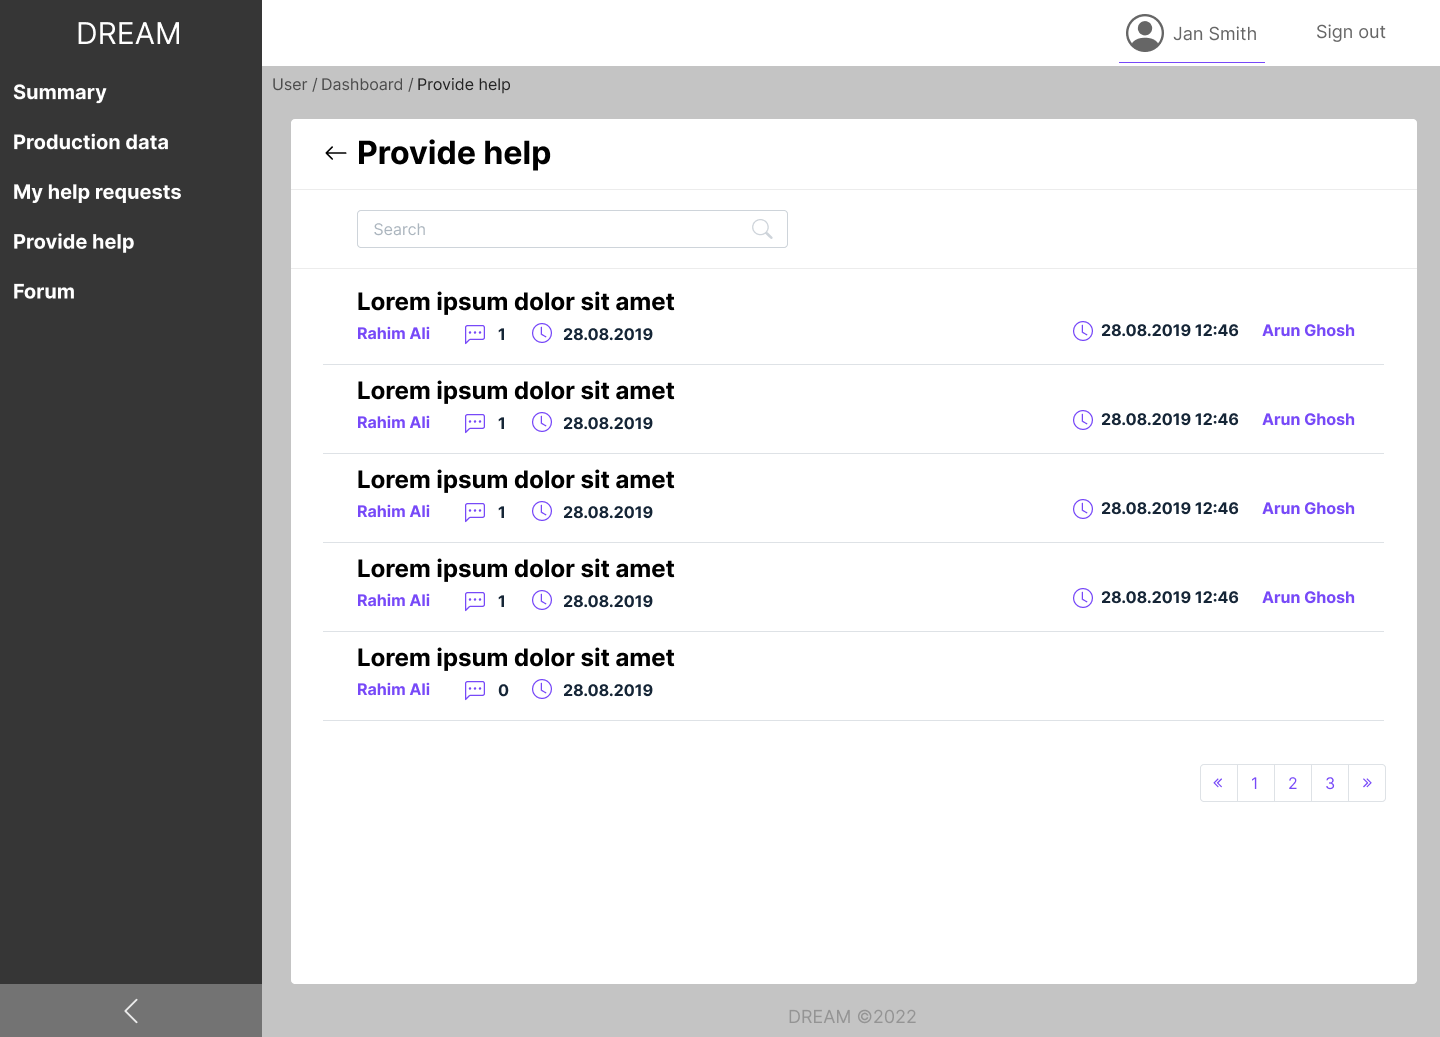
\includegraphics[width=0.75\textwidth]{mockups/Farmer_Dashboard_Provide help.png}
    \caption{\textbf{M12.} Help requests received by farmer with positive note.}
\end{figure}

\begin{figure}[H]
    \centering
    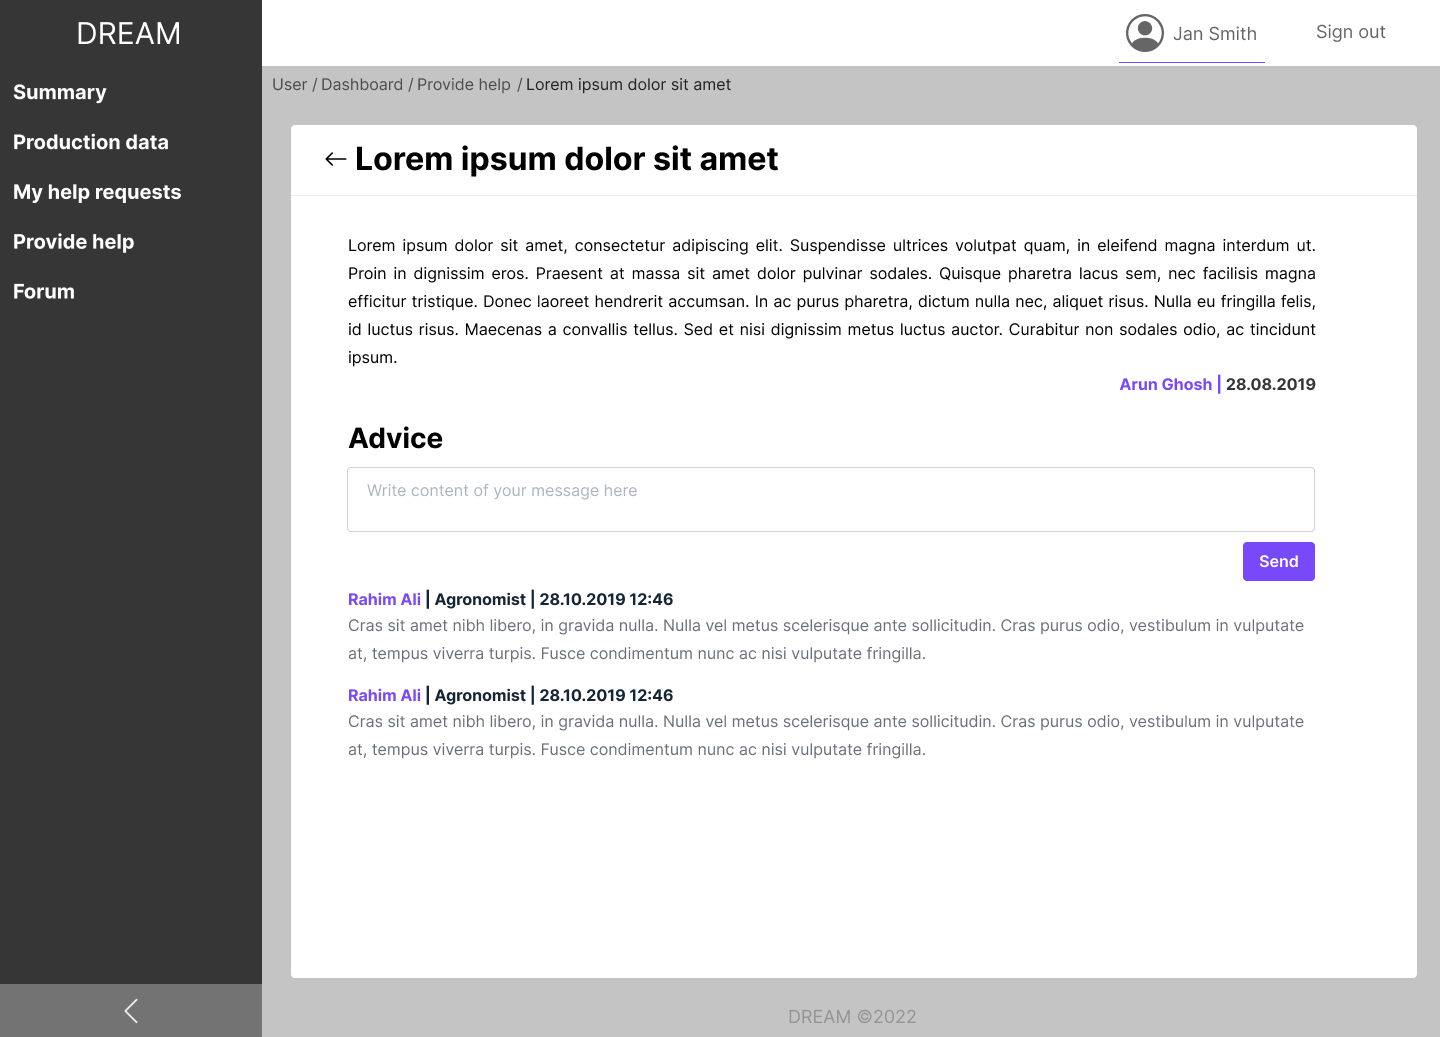
\includegraphics[width=0.75\textwidth]{mockups/Farmer_Dashboard_Provide help_Request.png}
    \caption{\textbf{M13.} Specific help request received by farmer with positive note (applicable also for the agronomist).}
\end{figure}

\begin{figure}[H]
    \centering
    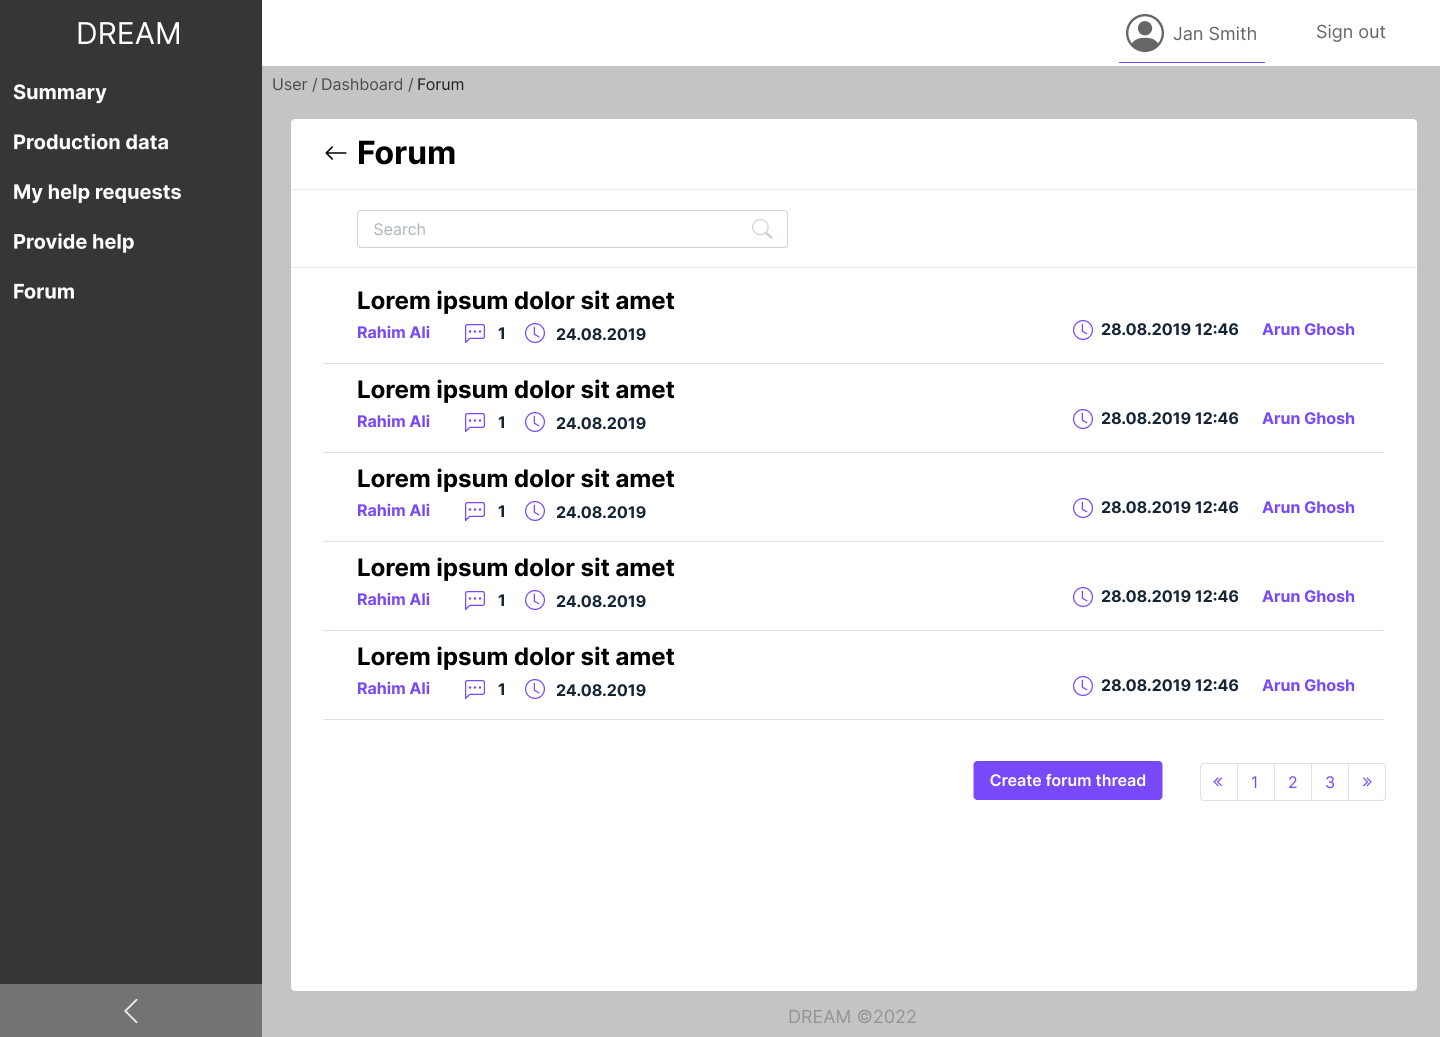
\includegraphics[width=0.75\textwidth]{mockups/Farmer_Dashboard_Forum.png}
    \caption{\textbf{M14.} Forum view.}
\end{figure}

\begin{figure}[H]
    \centering
    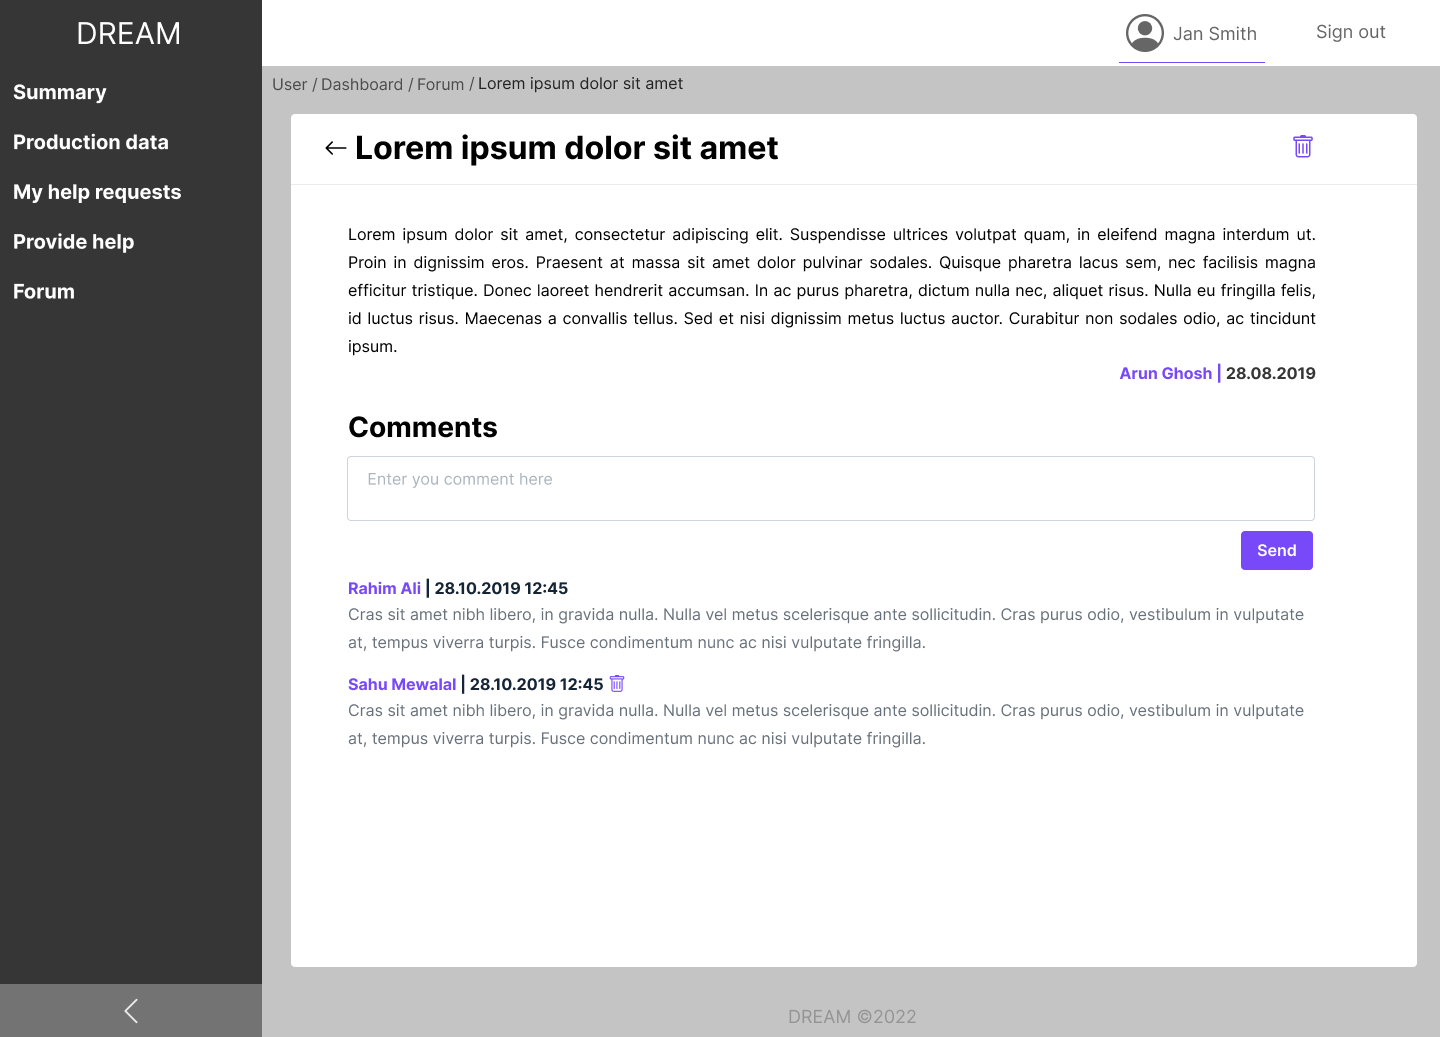
\includegraphics[width=0.75\textwidth]{mockups/Farmer_Dashboard_Forum_Thread.png}
    \caption{\textbf{M15.} Specific forum thread.}
\end{figure}

\begin{figure}[H]
    \centering
    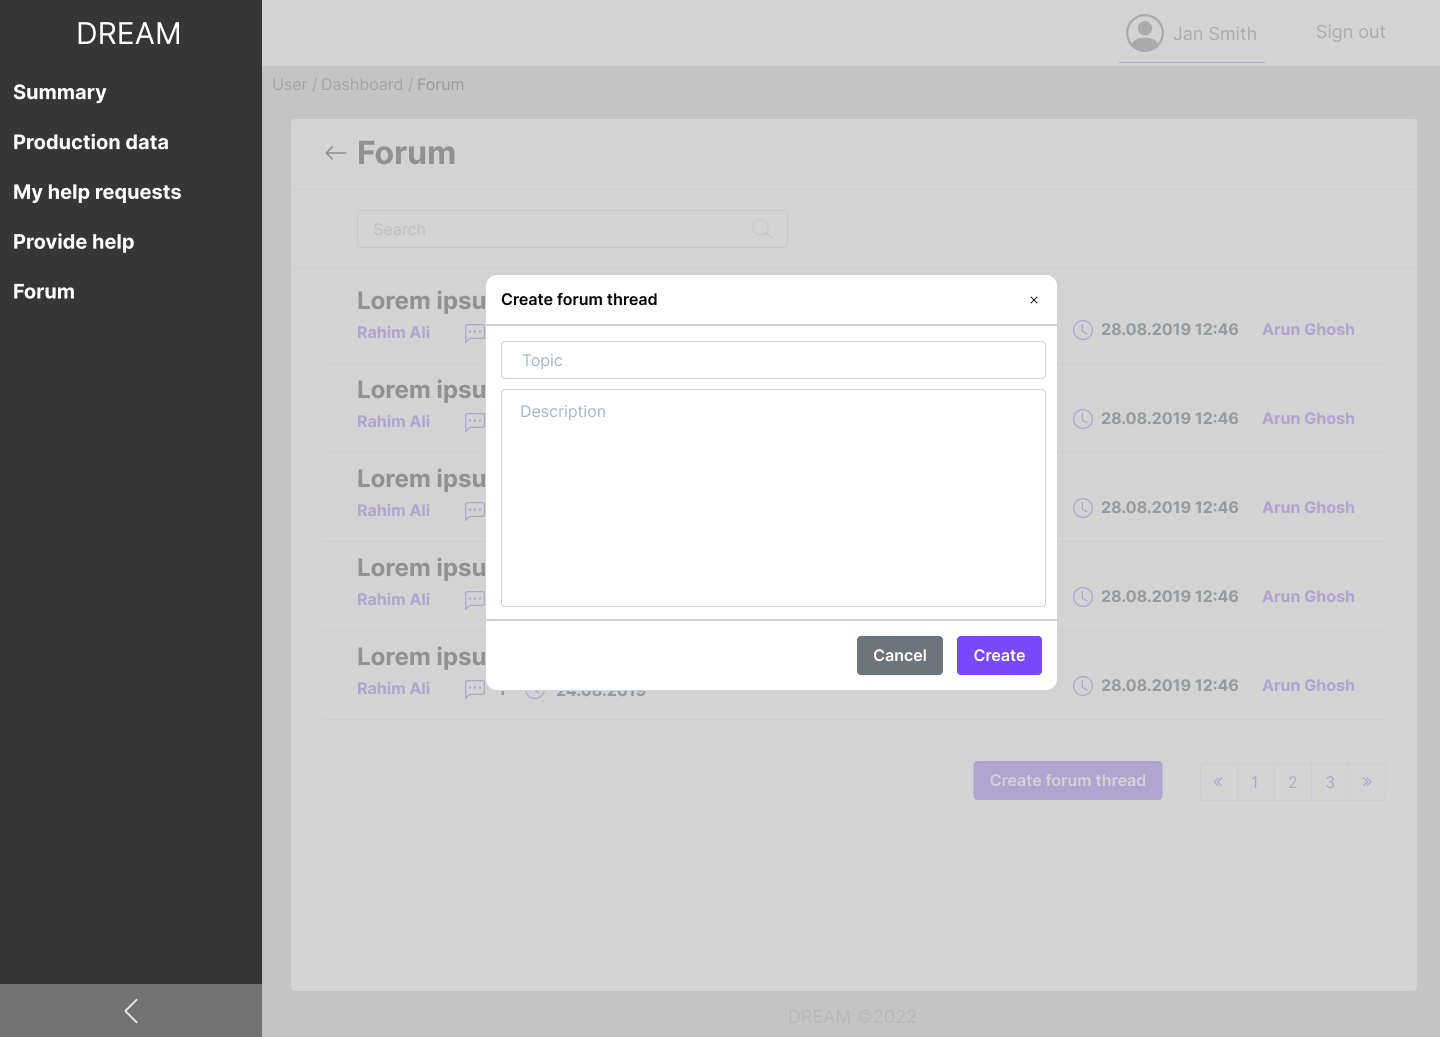
\includegraphics[width=0.75\textwidth]{mockups/Farmer_Dashboard_Forum_Create thread.png}
    \caption{\textbf{M16.} Creating forum thread.}
\end{figure}


\subsubsection{Agronomist}

\begin{figure}[H]
    \centering
    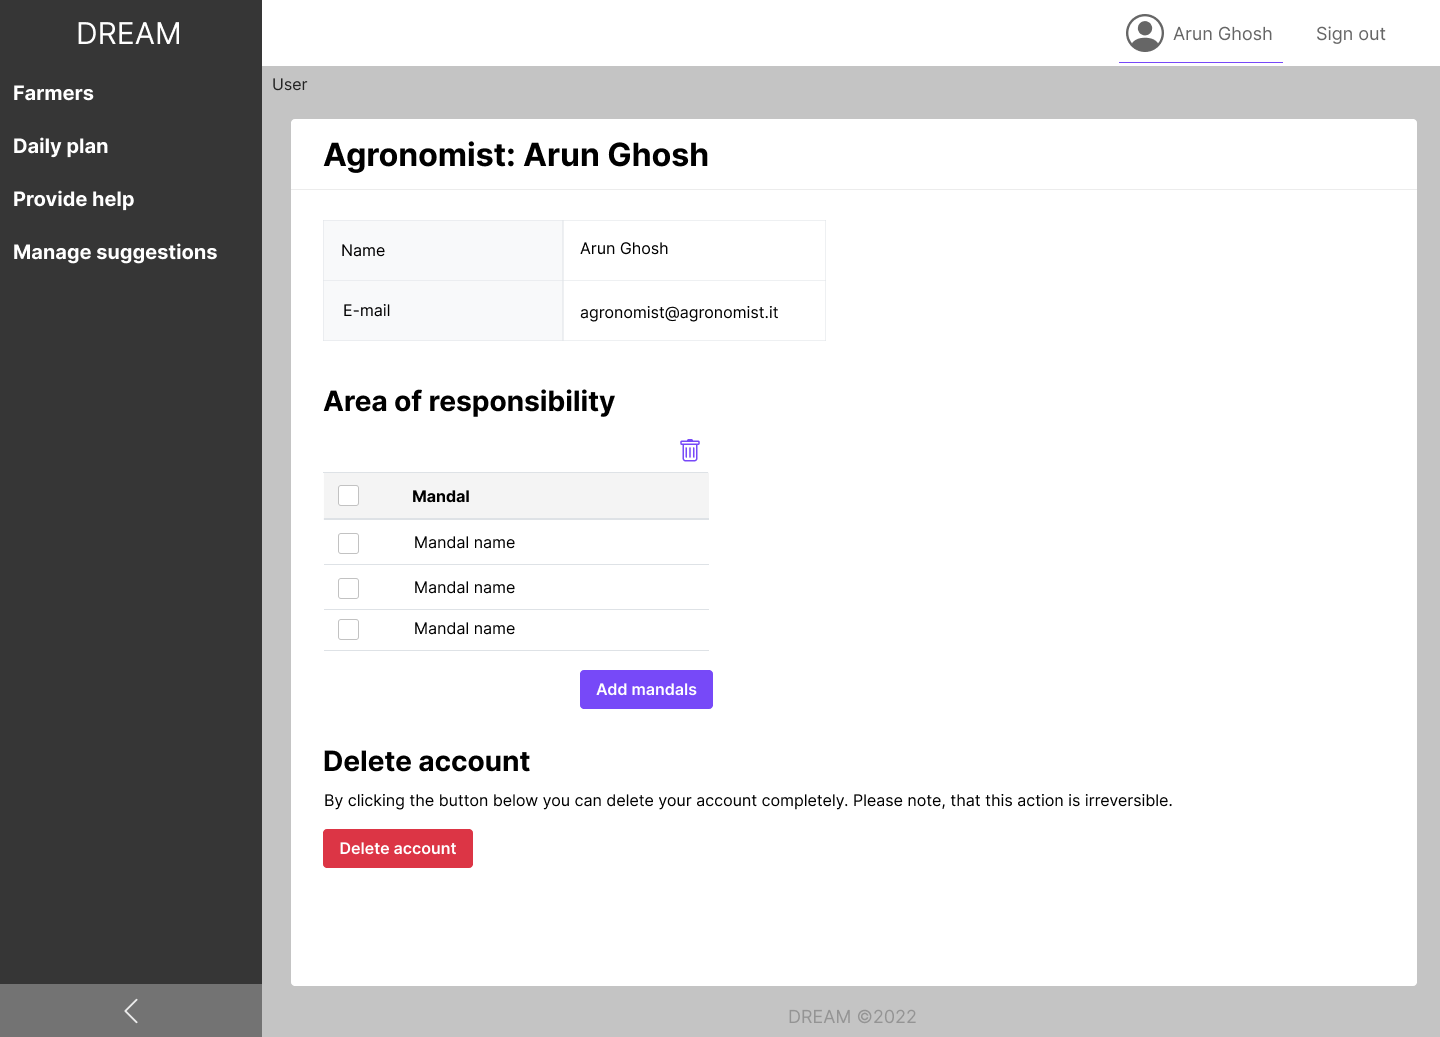
\includegraphics[width=0.75\textwidth]{mockups/Agronomist_User.png}
    \caption{\textbf{M17.} Agronomist's user view.}
\end{figure}

\begin{figure}[H]
    \centering
    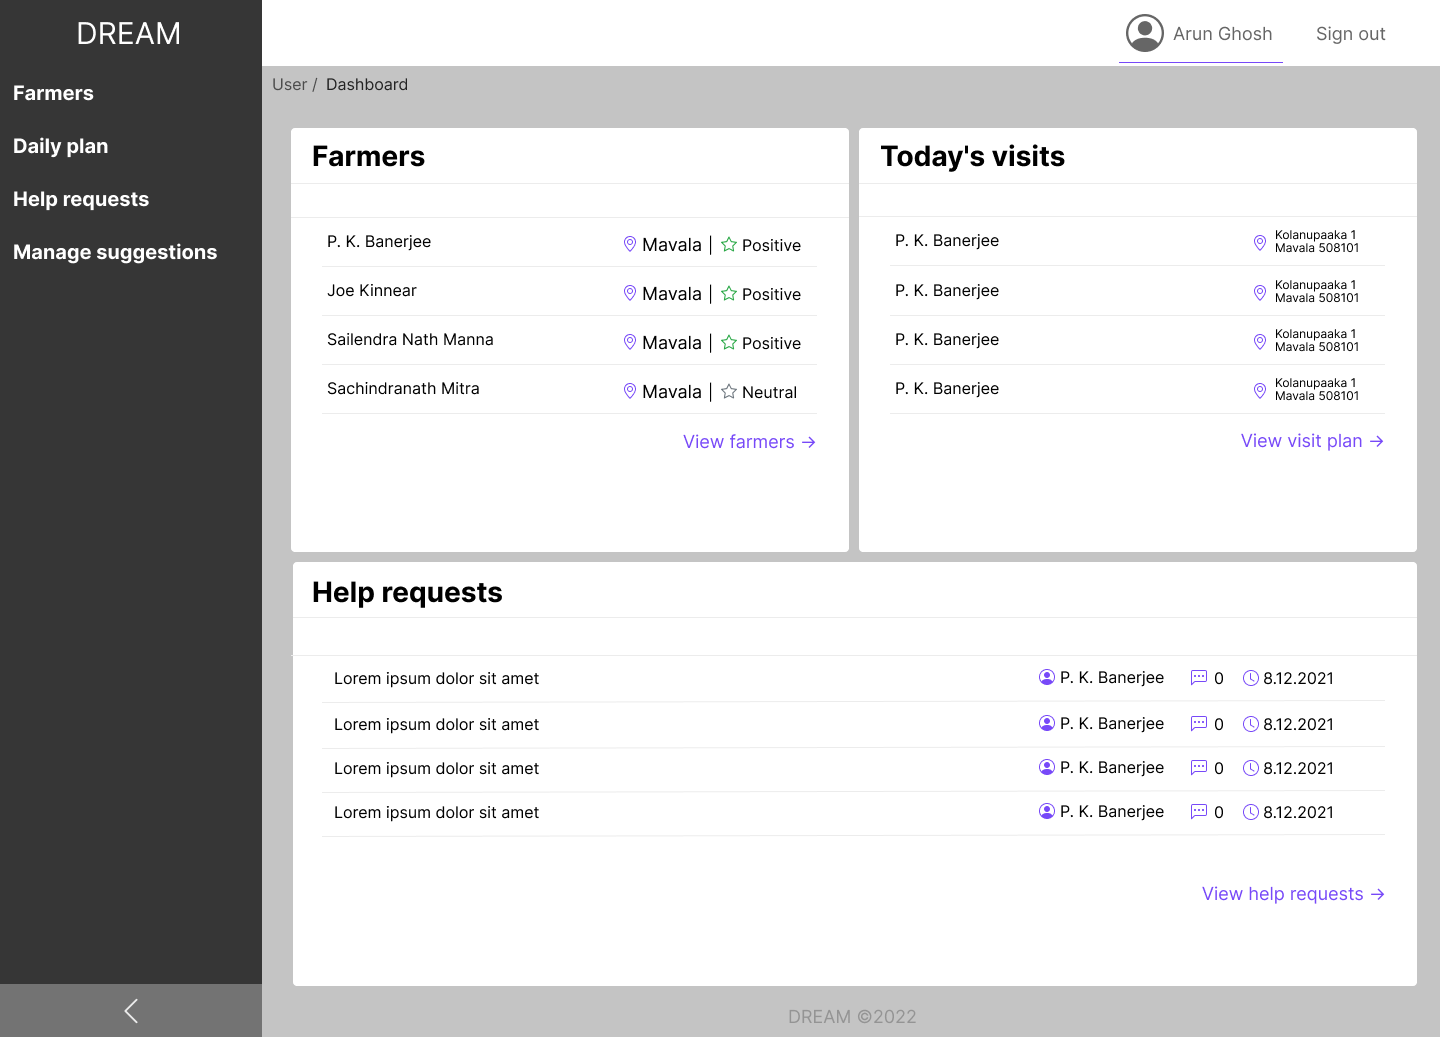
\includegraphics[width=0.75\textwidth]{mockups/Agronomist_Dashboard.png}
    \caption{\textbf{M18.} Agronomist's dashboard.}
\end{figure}

\begin{figure}[H]
    \centering
    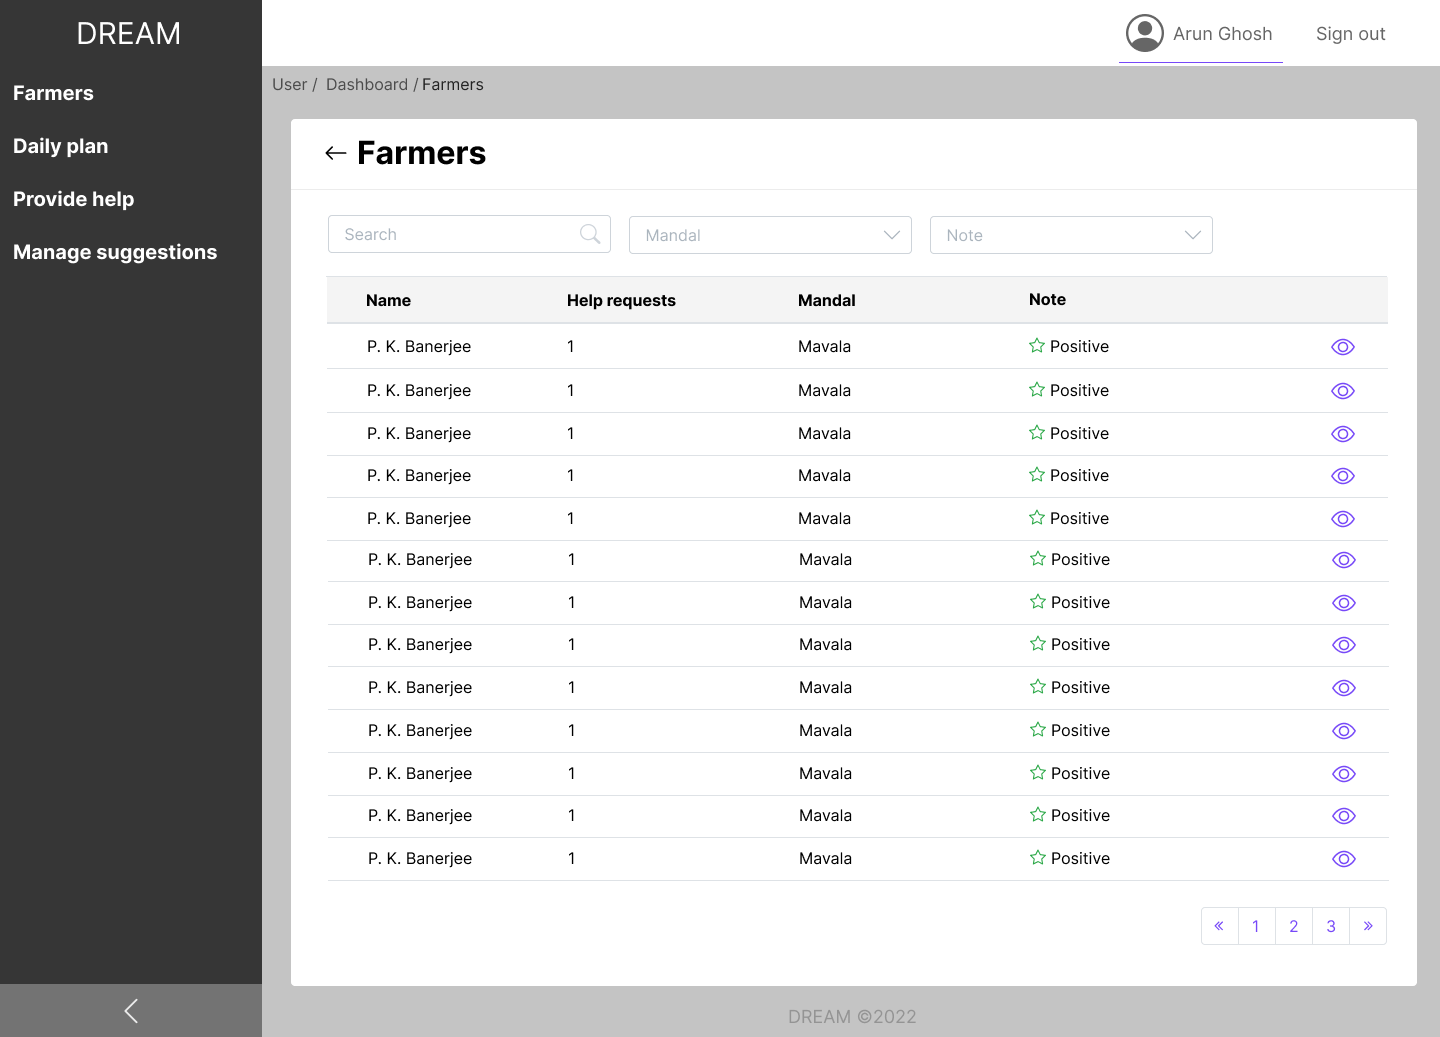
\includegraphics[width=0.75\textwidth]{mockups/Agronomist_Dashboard_Farmers.png}
    \caption{\textbf{M19.} List of farmers (applicable also for the policy maker).}
\end{figure}

\begin{figure}[H]
    \centering
    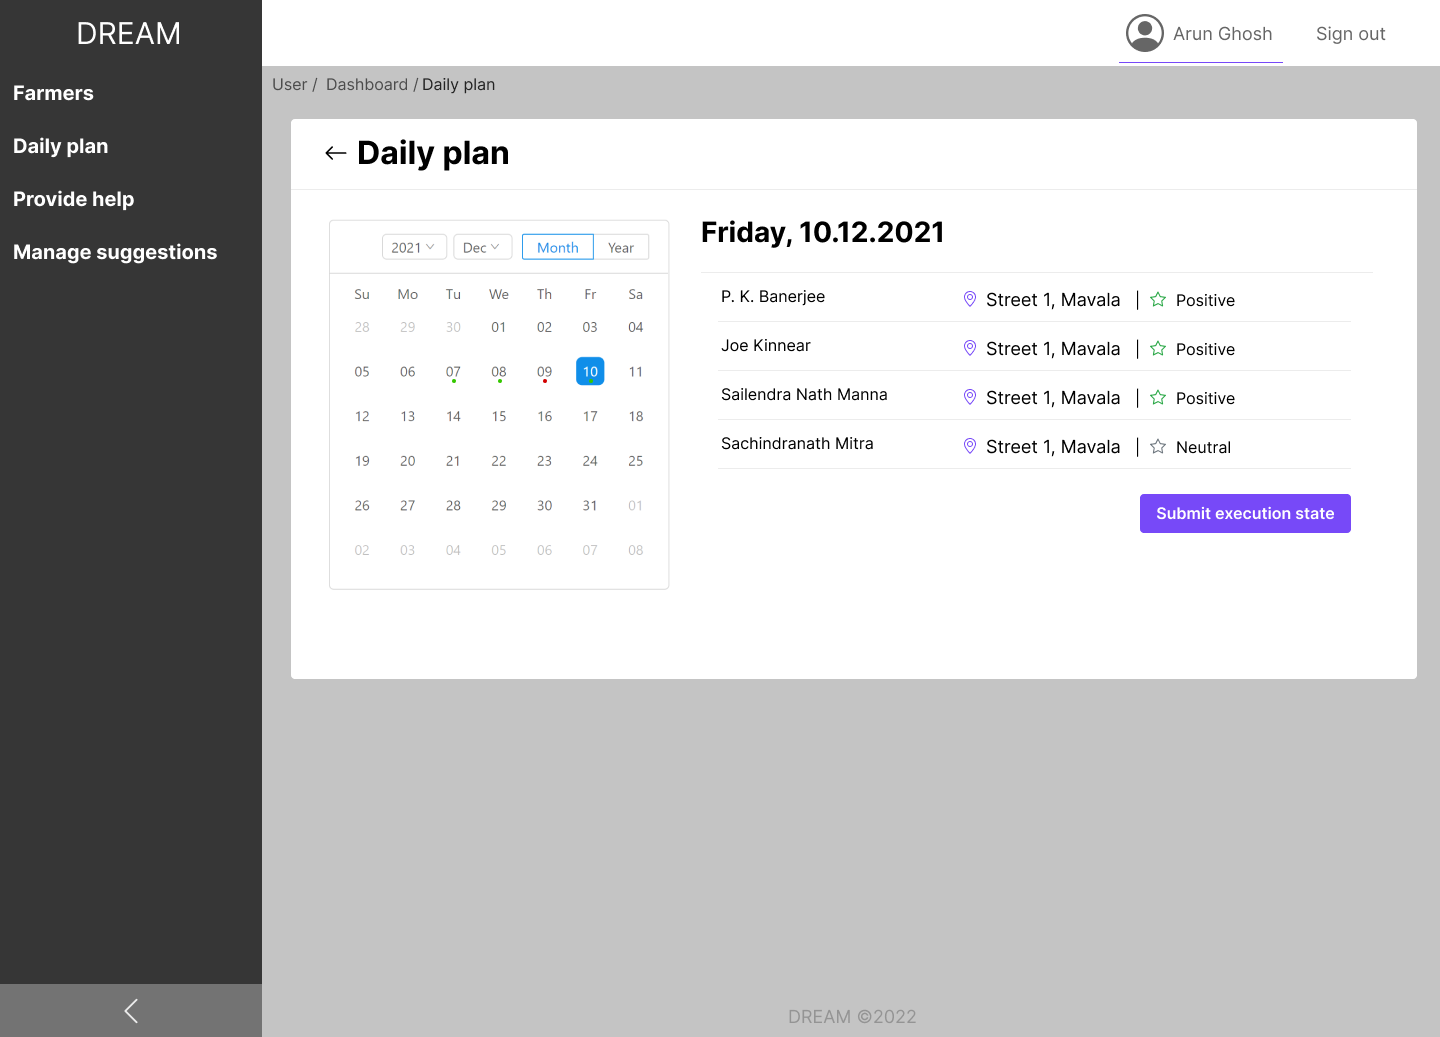
\includegraphics[width=0.75\textwidth]{mockups/Agronomist_Dashboard_Visit plan.png}
    \caption{\textbf{M20.} Calendar of daily plans.}
\end{figure}

\begin{figure}[H]
    \centering
    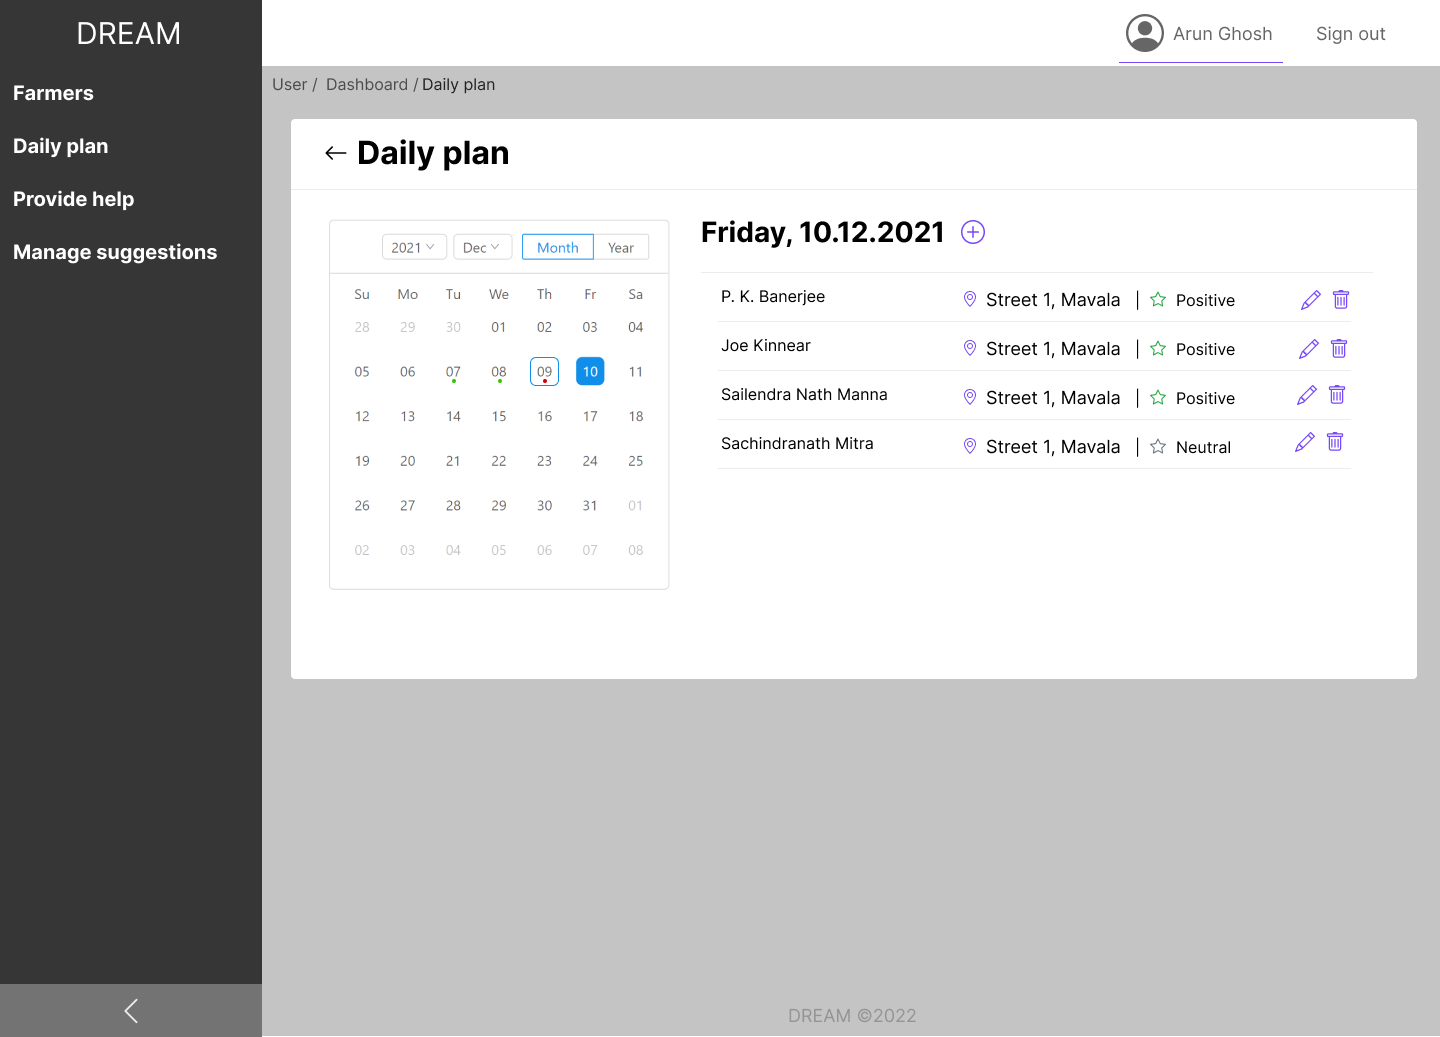
\includegraphics[width=0.75\textwidth]{mockups/Agronomist_Dashboard_Visit plan in future.png}
    \caption{\textbf{M21.} Calendar of daily plans – view of future day.}
\end{figure}

\begin{figure}[H]
    \centering
    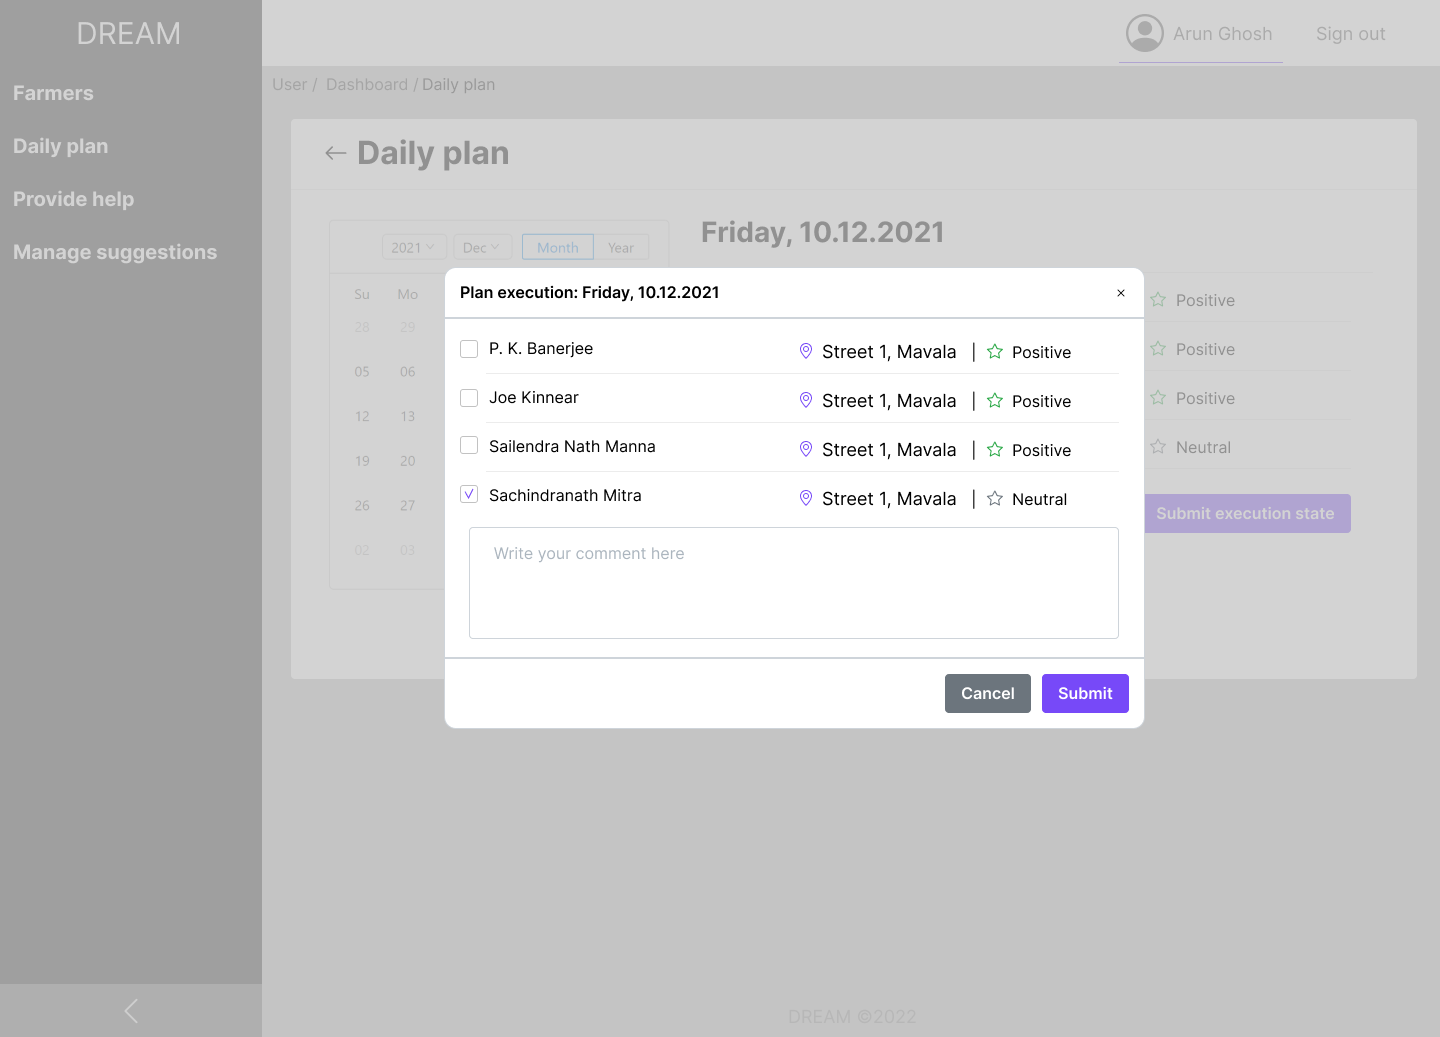
\includegraphics[width=0.75\textwidth]{mockups/Agronomist_Dashboard_Visit plan_Submit.png}
    \caption{\textbf{M22.} Submitting executions state of a daily plan.}
\end{figure}

\begin{figure}[H]
    \centering
    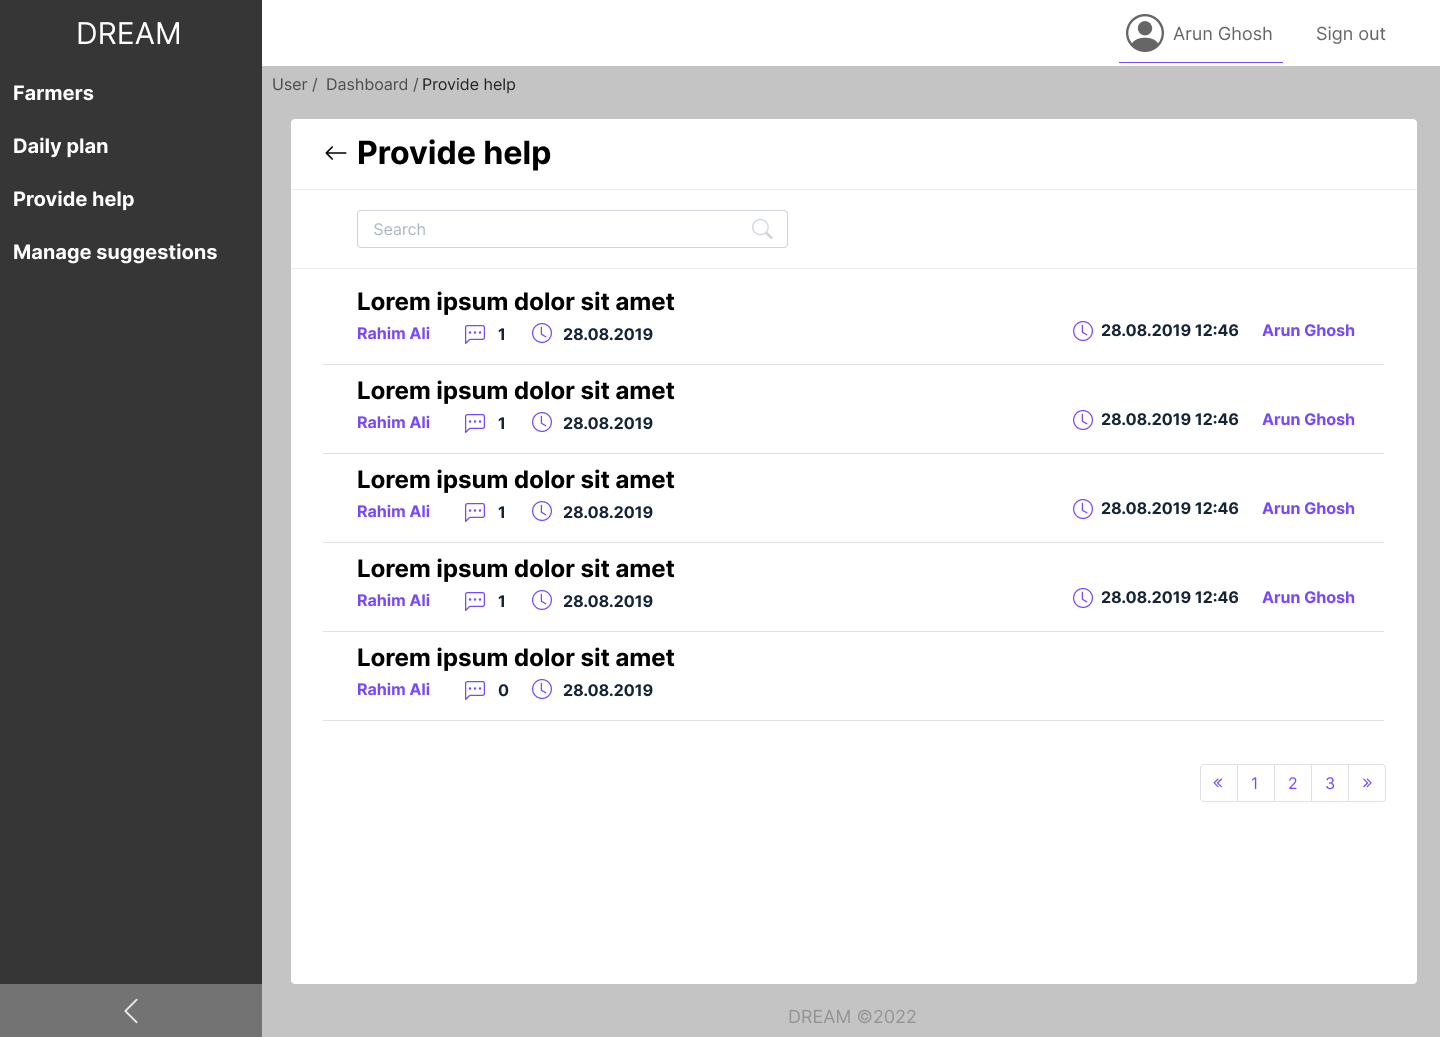
\includegraphics[width=0.75\textwidth]{mockups/Agronomist_Dashboard_Provide help.png}
    \caption{\textbf{M23.} Help requests received by agronomist.}
\end{figure}

\begin{figure}[H]
    \centering
    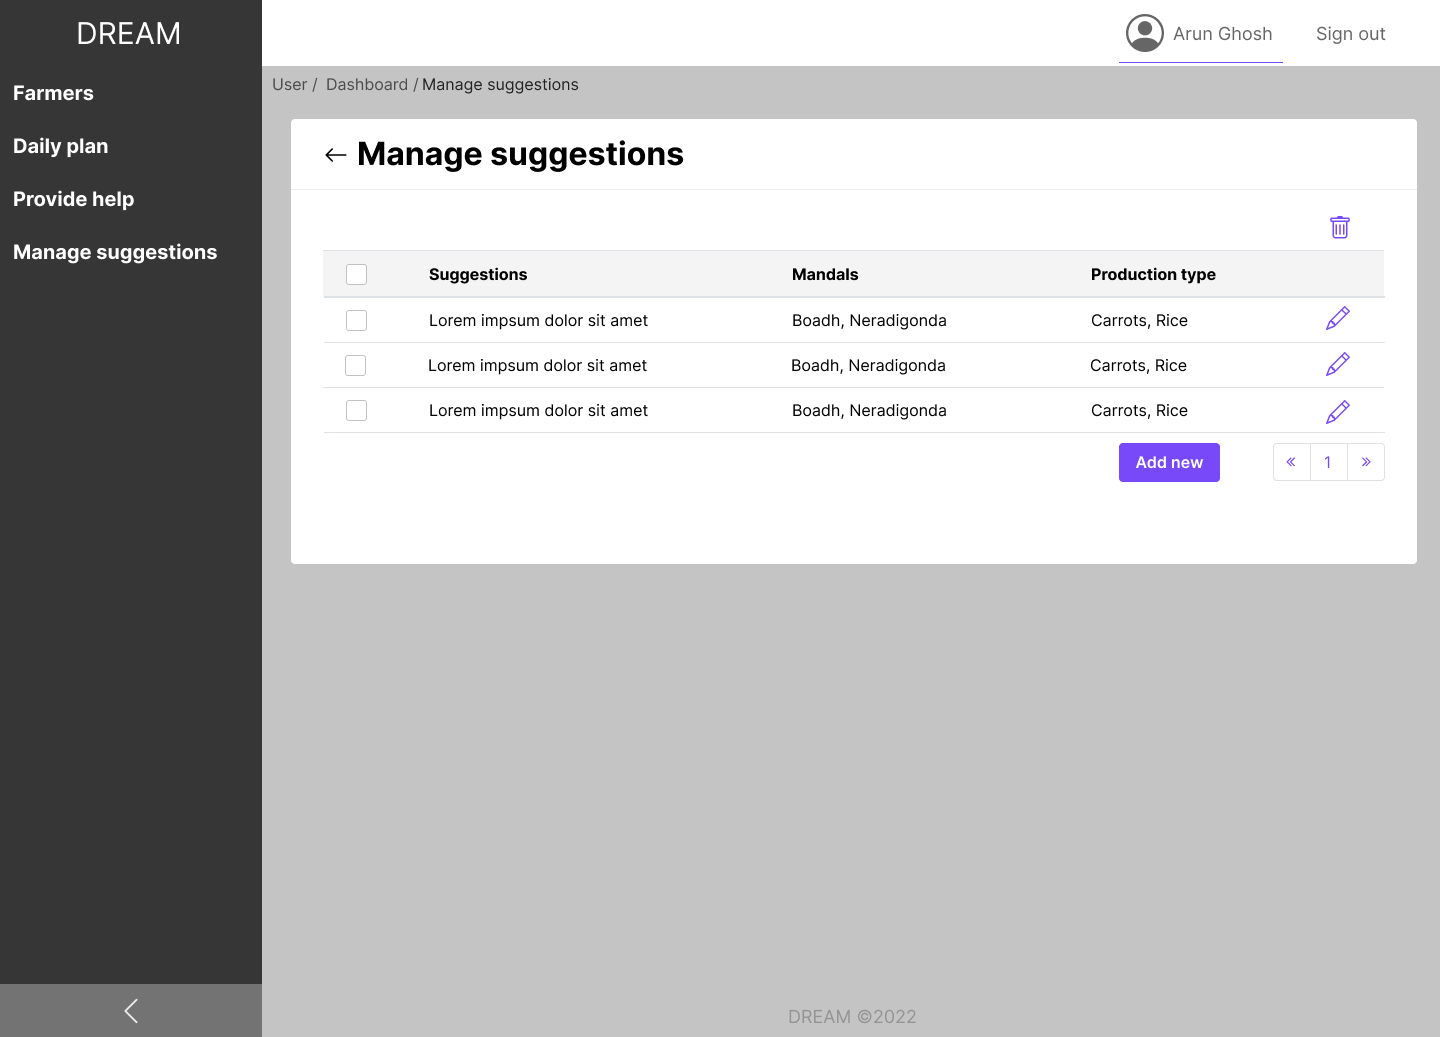
\includegraphics[width=0.75\textwidth]{mockups/Agronomist_Dashboard_Manage suggestions.png}
    \caption{\textbf{M24.} Managing suggestions.}
\end{figure}

\subsubsection{Policy maker}

\begin{figure}[H]
    \centering
    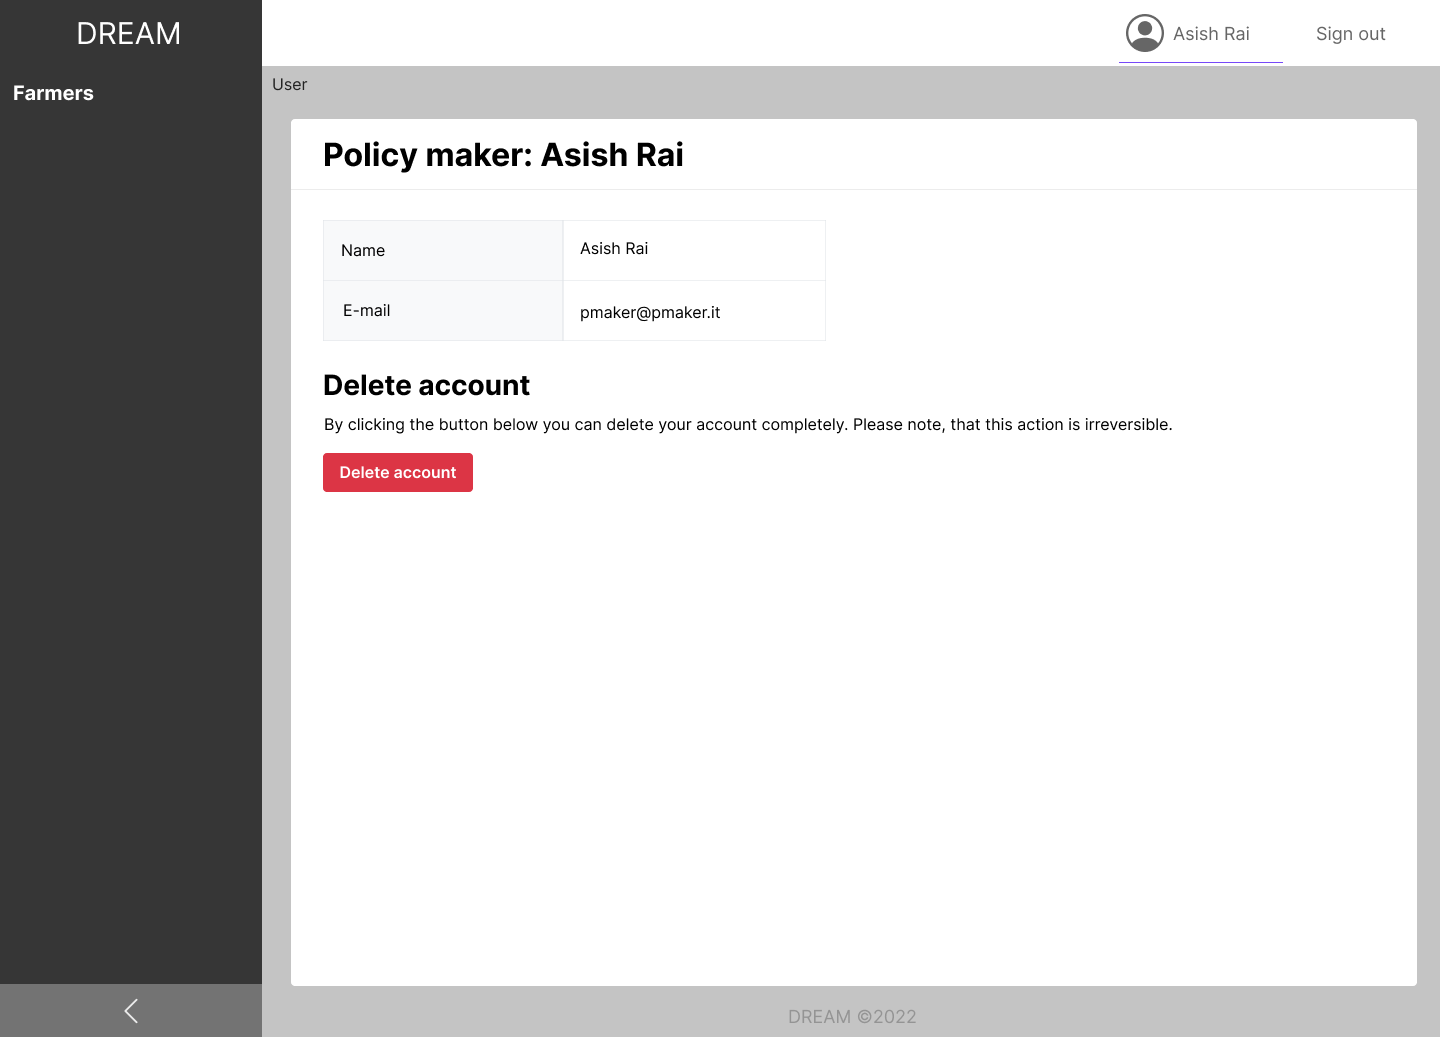
\includegraphics[width=0.75\textwidth]{mockups/Policy maker_User.png}
    \caption{\textbf{M25.} Policy maker's user view.}
\end{figure}

\begin{figure}[H]
    \centering
    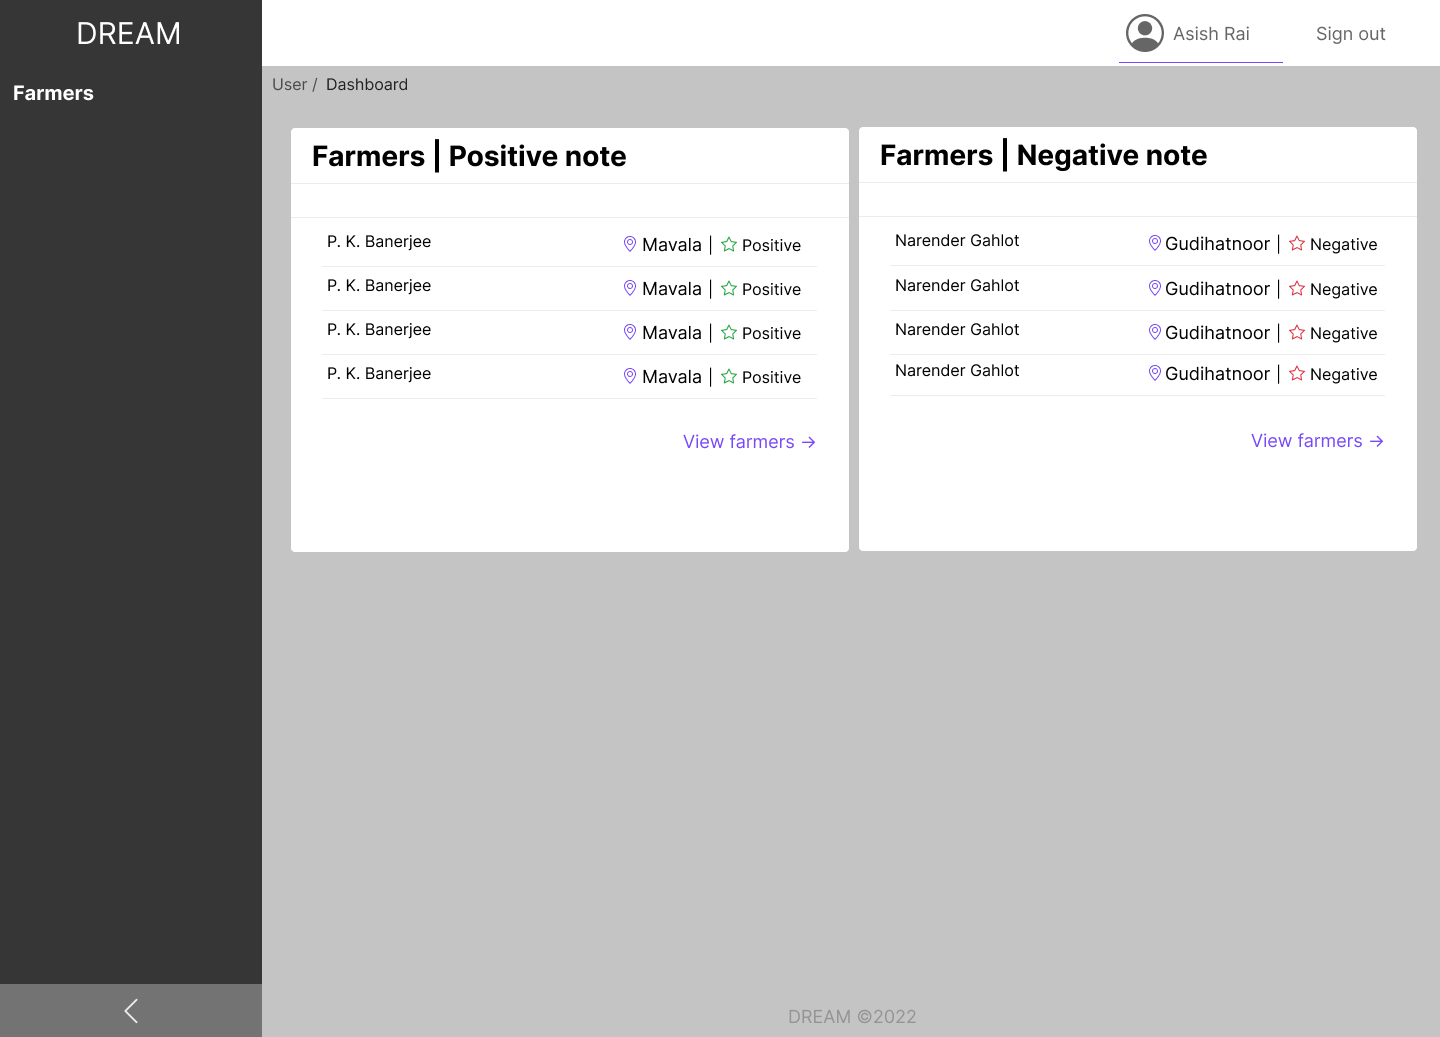
\includegraphics[width=0.75\textwidth]{mockups/Policy maker_Dashboard.png}
    \caption{\textbf{M26.} Policy maker's dashboard.}
\end{figure}

\begin{figure}[H]
    \centering
    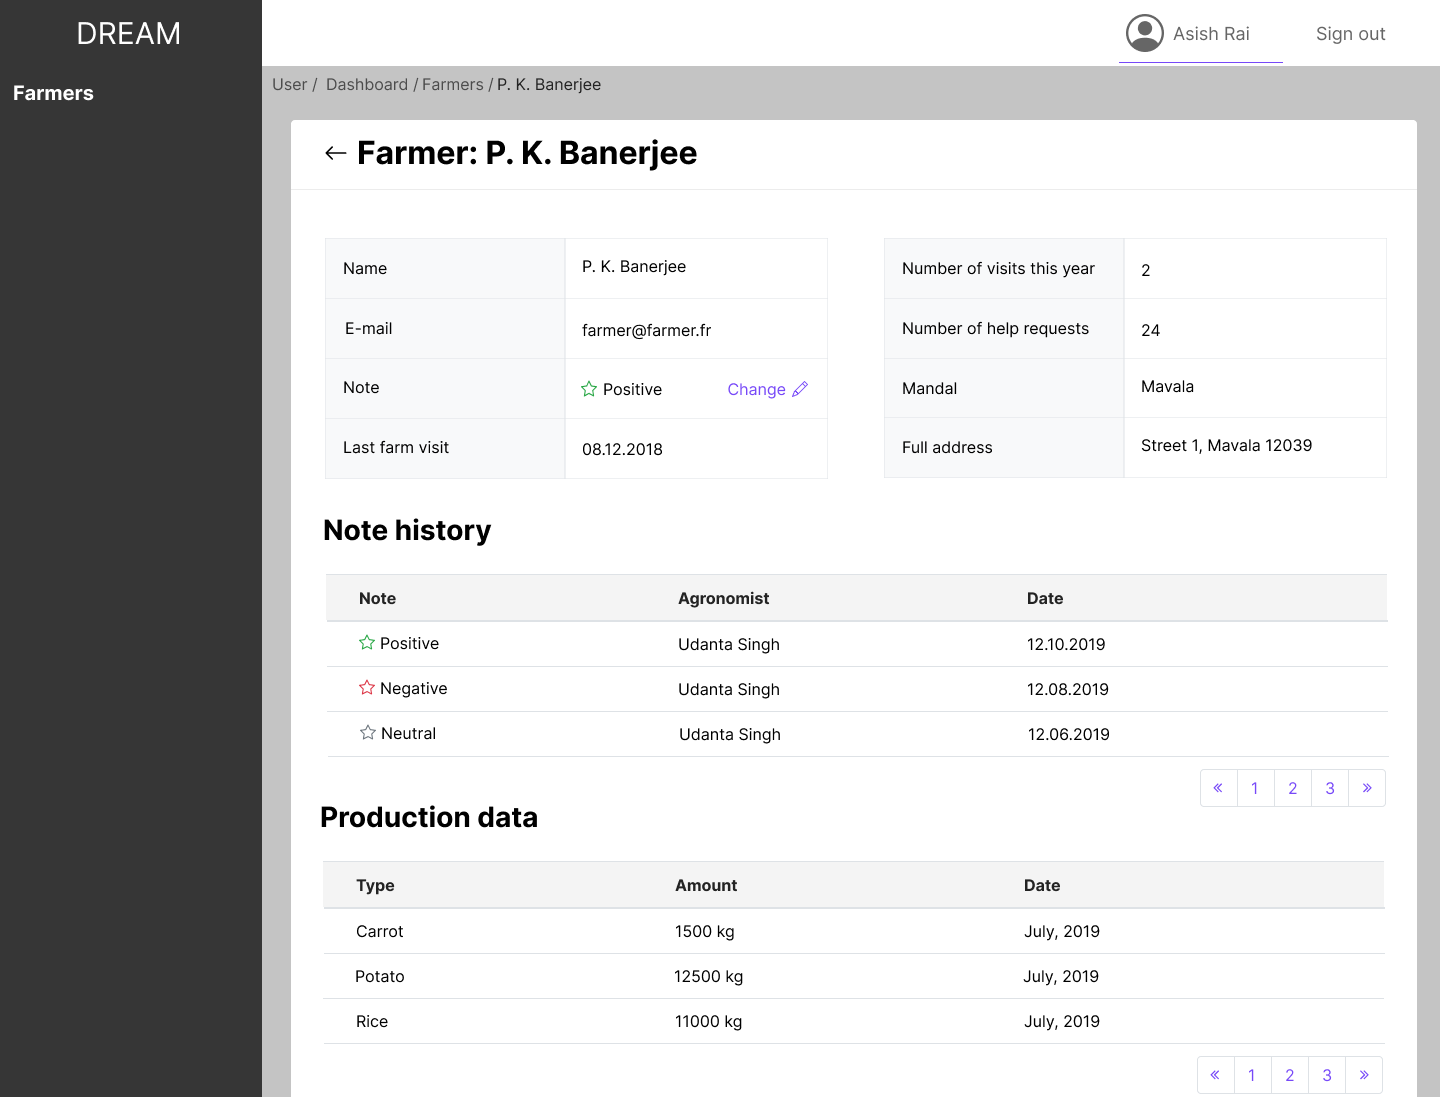
\includegraphics[width=0.75\textwidth]{mockups/Policy maker_Dashboard_Farmers_Farmer_part1.png}
    \caption{\textbf{M27.} Partial view of farmer's summary (applicable also to agronomist, without option to change note)}
\end{figure}

\begin{figure}[H]
    \centering
    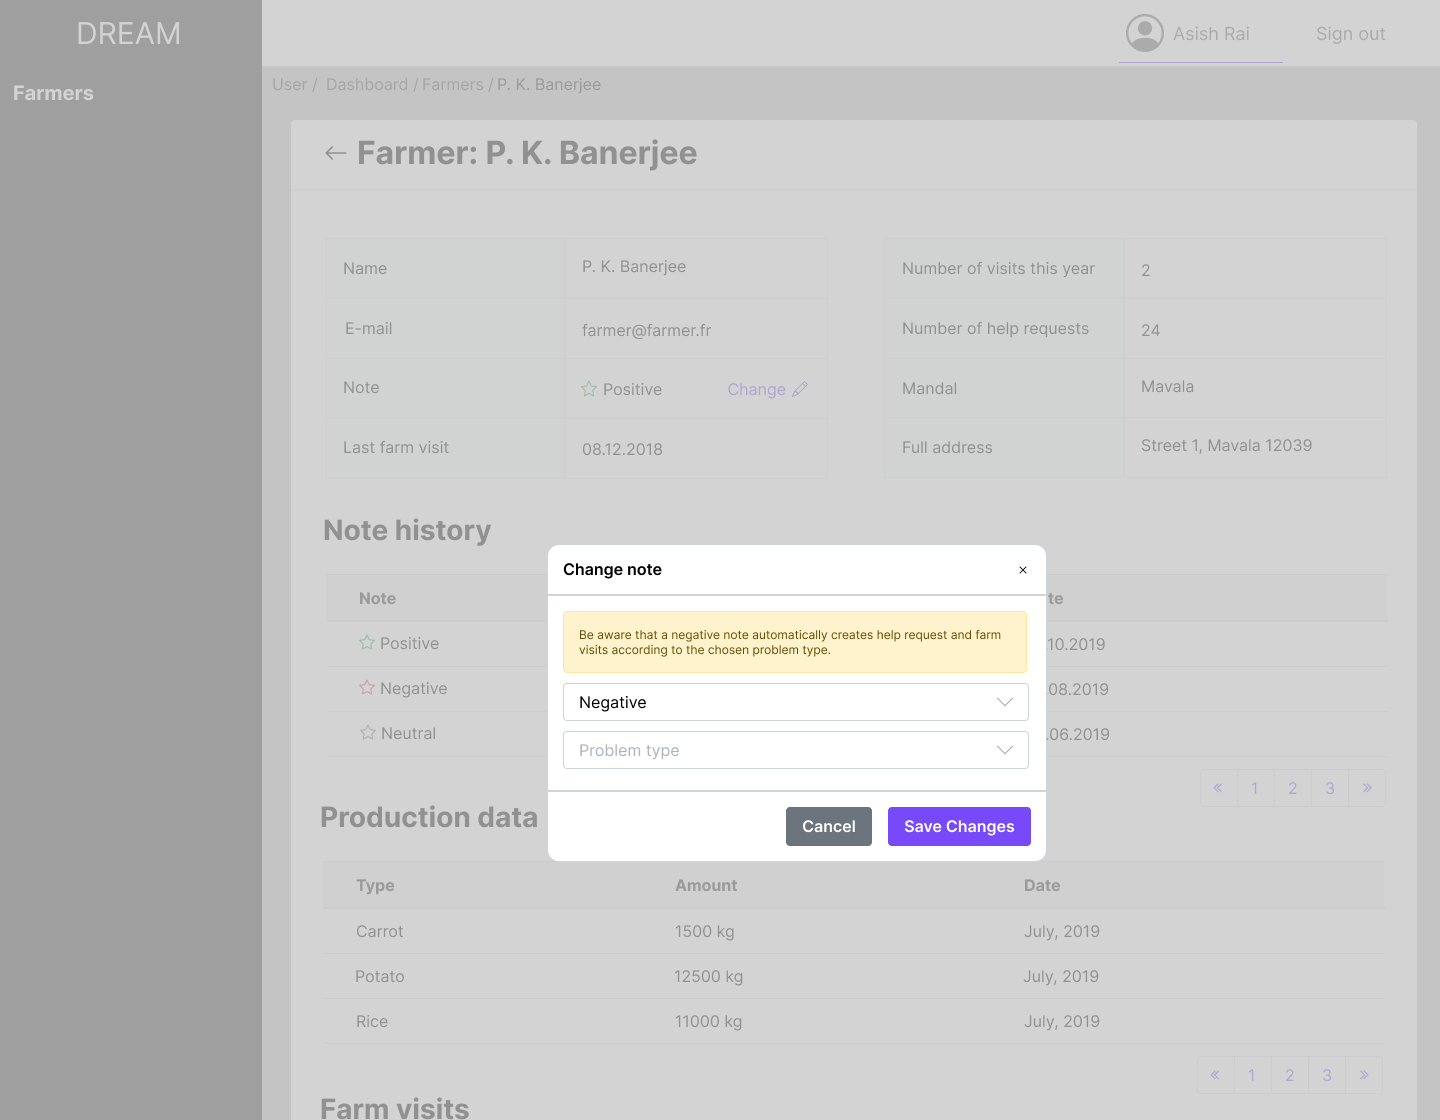
\includegraphics[width=0.75\textwidth]{mockups/Policy maker_Dashboard_Farmers_Farmer_Note_1.png}
    \caption{\textbf{M28.} Assigning note to farmer.}
\end{figure}
